\documentclass{article}
\usepackage[utf8]{inputenc}
\usepackage{polski}
\usepackage{titling}
\usepackage{graphicx}

\usepackage{placeins}
\usepackage{subcaption}
\usepackage{amsmath}

\usepackage{hyperref}

\usepackage{indentfirst}


\usepackage{listings}
\usepackage{xcolor}

%New colors defined below
\definecolor{codegreen}{rgb}{0,0.6,0}
\definecolor{codegray}{rgb}{0.5,0.5,0.5}
\definecolor{codepurple}{rgb}{0.58,0,0.82}
\definecolor{backcolour}{rgb}{0.95,0.95,0.92}

%Code listing style named "mystyle"
\lstdefinestyle{mystyle}{
  backgroundcolor=\color{backcolour},  
  commentstyle=\color{codegreen},
  keywordstyle=\color{magenta},
  numberstyle=\tiny\color{codegray},
  stringstyle=\color{codepurple},
  basicstyle=\ttfamily\footnotesize,
  breakatwhitespace=false,         
  breaklines=true,                 
  captionpos=b,                    
  keepspaces=true,                 
  showspaces=false,                
  showstringspaces=false,
  showtabs=false,                  
  tabsize=2
}
\lstset{style=mystyle}


\newcommand{\subtitle}[1]{%
  \posttitle{%
    \par\end{center}
    \begin{center}\large#1\end{center}
    \vskip0.5em}%
} 

\title{\textbf{TAP} \\ Technika Automatyzacji Procesów}
\subtitle{Regulator PID i MPCS}
\author{Kacper Michalski, Paweł Rawicki }
\date{Lipiec 2021}

\author{Kacper Michalski Paweł Rawicki }
\date{Maj 2021}

\begin{document}

\maketitle


\newpage 
\tableofcontents

\newpage
\section{Opis Zadania}
\begin{figure}[h!]
    \centering
\includegraphics[width=1\linewidth]{img/introduction/TAPtask1.pdf}
\end{figure}
\newpage{}
\section{Regulator PI bez odsprzęgania}
\indent Regulator PI z odsprzęganiem radzi sobie zadowalająco na zadanych przebiegach. Widać ewidentny wpływ zmiany wartości zadanej jednego wyjścia na wyjście drugie.

\subsection{Dobrane nastawy regulatora PI}
\indent Dobieranie nastaw regulatora PI zostało wykonane metodą heurystyczną, kierując się charakterystykami otrzymanych sygnałów sterowania i wyjściowych oraz również dążąc do minimalizacji błędów kwadratowych, tak by osiągnąć kompromis pomiędzy tymi wskaźnikami \\
\indent Wskaźnik jakości był wyliczany w następujący sposób dla przykładowych trajektorii zadanych:
\begin{lstlisting}[language=Matlab]
    e=rVector(ct,:) - y; % wartosc zadana- wyjscie
    errorH=e(1)^2;  
    errorT=e(2)^2;        
\end{lstlisting}

\indent Na regulator nałożono także następujące ograniczenia na minimalną i maksymalną wartość sterowania taką samą dla obu regulatorów:\\
$U_min=0$  $U_max=300$ \\

\indent W regulatorze działa także mechanizm anti windup zaczerpnięty z \href {https://www.mathworks.com/matlabcentral/answers/642205-how-do-i-set-the-saturation-output-for-pid-objects-in-matlab}{link}


\indent Dobrane parametry są następujące: \\
$KpFh=0.9$   $KiFh=0.01$ \\
$KpFcin= -0.2$  $ KiFcin2=-0.002$ \\

\subsection{PI dla przykładowych przebiegów z obiektem nielinowym}
\indent Na poniższych wykresach zostały przedstawione przykładowe przebiegi dla różnych wartości zadanych. Wyliczane wartości sterowania były podawana na model nieliniowy obiektu. \\
\indent Można zaobserwować, że zmiana jednej wartości zadanej dla jednego wyjścia wpływa na wyjście drugie. Spowodowane jest to głównie opóźnieniami w obiekcie, które sprawiają, ż regulator potrzebuje czasu aby się dostosować. \\
\indent Widać też, że regulator sobie nie radzi dla przypadku gdy temperatura zadana jest bliska temperaturze zimnej wody. Występuje wtedy uchyb na temperaturze, zaś wysokość cieczy rośnie. Pokazuje to ograniczenia regulatora oraz to, że zadawanie wartości skrajnych lub poza zakresem pracy może być niebezpieczne dla obiektu, gdy regulator ma jedne człony o większej wadze od innych. Tutaj przyczyną będzie całkowanie uchybu temperatury i zwiększanie dopływu zimnej wody oraz fakt, że cały czas jest dopływ zakłócenia o temperaturze wyższej niż temperatura zimnej wody.Czyli nie jest możliwe osiągnięcie zadanej temperatury, jednak regulator ciągle próbuje ją osiągnąć. Z tego powodu w realnym zastosowaniu należałoby podać zakres możliwych wartości zadanych, gdyż błąd operatora, wynikający z braku świadomości wpływu zakłócenia, może zniszczyć układ. 

\FloatBarrier
    \begin{figure}[h!]
   \centering
   \begin{subfigure}[b]{0.4\textwidth}
      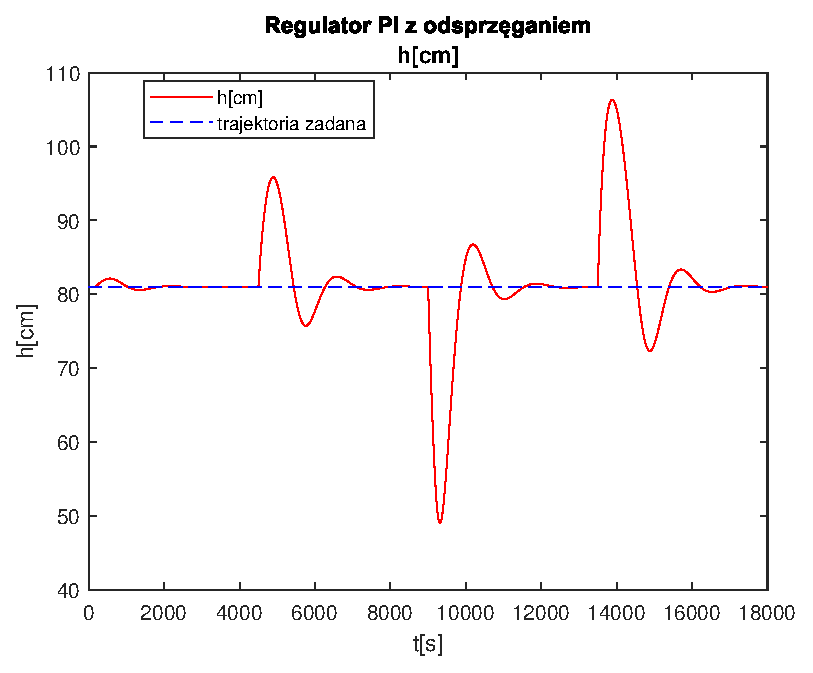
\includegraphics[width=1\linewidth]{img/PI/decoupler/disturbance/PIDecouplerH2DisttrueLinfalse.eps}
      \caption{}
      \label{fig:fig:PIDecoupler2DisttrueLinfalse1}
   \end{subfigure}
       
   \begin{subfigure}[b]{0.4\textwidth}
      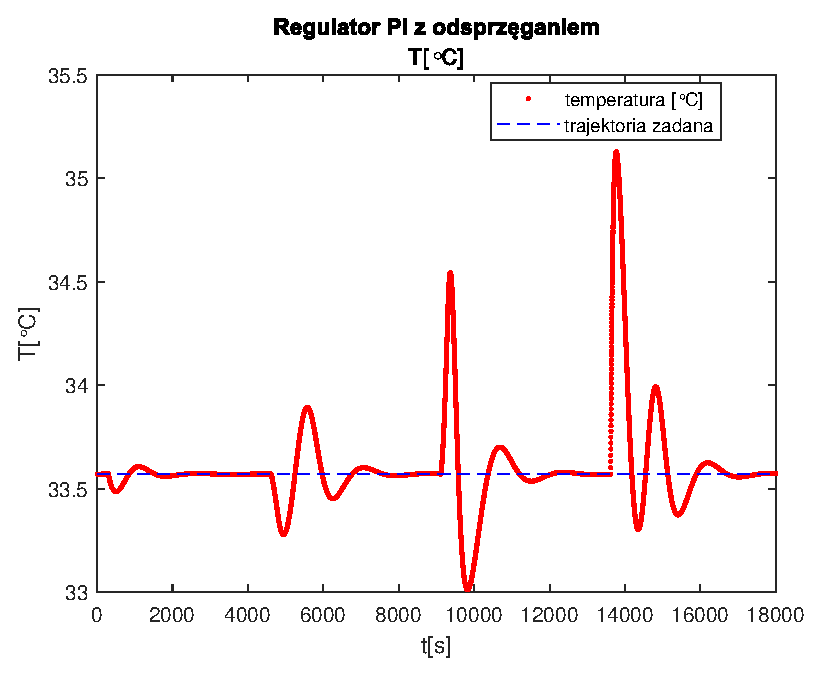
\includegraphics[width=1\linewidth]{img/PI/decoupler/disturbance/PIDecouplerT2DisttrueLinfalse.eps}
      \caption{}
      \label{fig:fig:PIDecoupler2DisttrueLinfalse2}
   \end{subfigure}
       
   \begin{subfigure}[b]{0.4\textwidth}
      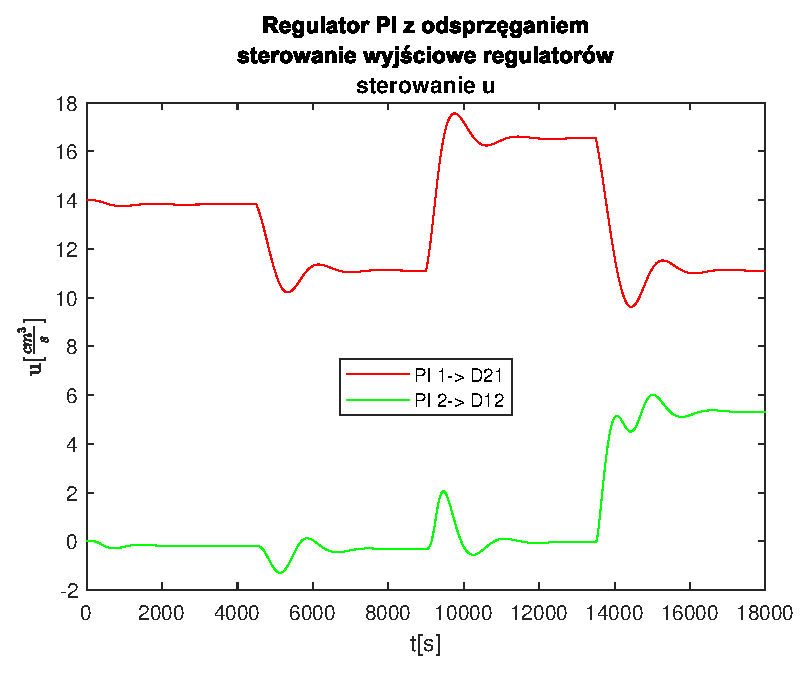
\includegraphics[width=1\linewidth]{img/PI/decoupler/disturbance/PIDecouplerControlD2DisttrueLinfalse.eps}
      \caption{}
      \label{fig:fig:PIDecoupler2DisttrueLinfalse3}
   \end{subfigure}
       
   \begin{subfigure}[b]{0.4\textwidth}
      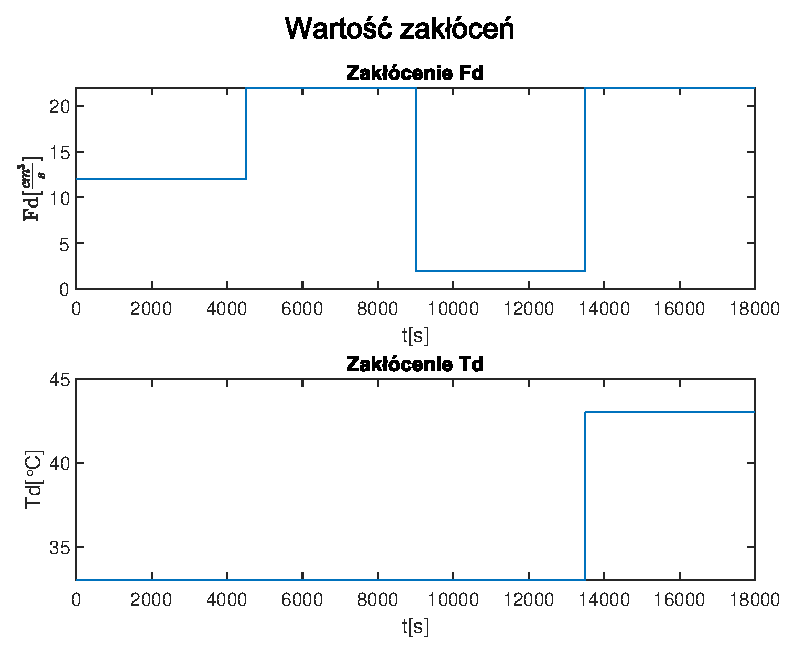
\includegraphics[width=1\linewidth]{img/PI/decoupler/disturbance/PIDecouplerDisturbance2DisttrueLinfalse.eps}
      \caption{}
      \label{fig:fig:PIDecoupler2DisttrueLinfalse4}
   \end{subfigure}
       
   \caption{Wykresy dla regulatora PI z odsprzeganiem dla różnych wartości zakłóceń}
   \label{fig:PIDecoupler2DisttrueLinfalse}
\end{figure}
           
\begin{figure}[h!]
   \centering
   \begin{subfigure}[b]{0.4\textwidth}
      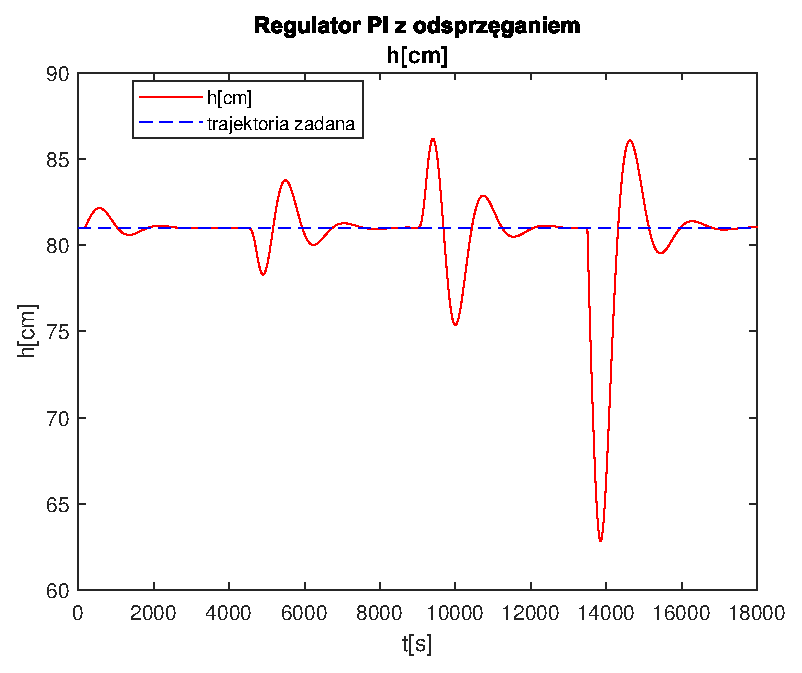
\includegraphics[width=1\linewidth]{img/PI/decoupler/disturbance/PIDecouplerH3DisttrueLinfalse.eps}
      \caption{}
      \label{fig:fig:PIDecoupler3DisttrueLinfalse1}
   \end{subfigure}
       
   \begin{subfigure}[b]{0.4\textwidth}
      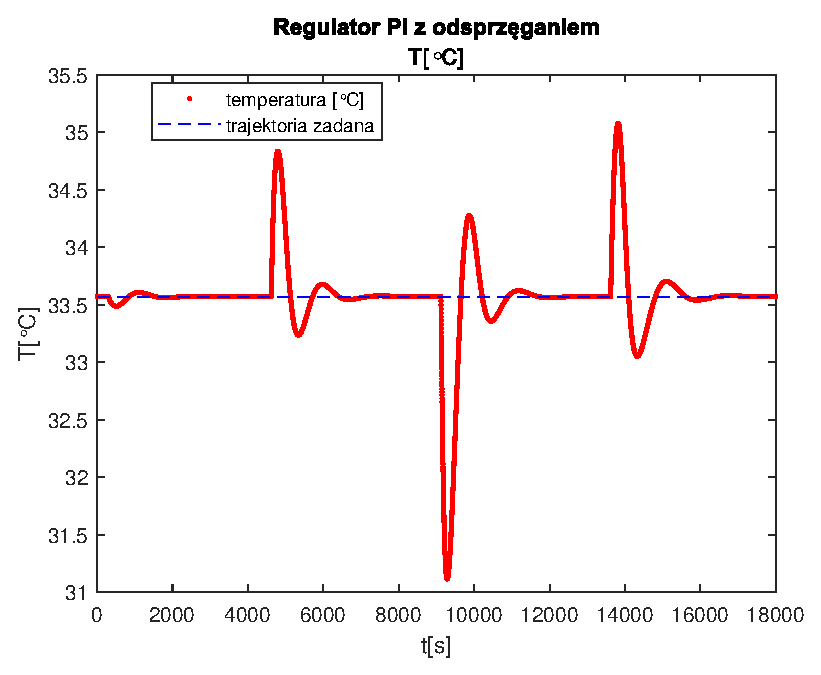
\includegraphics[width=1\linewidth]{img/PI/decoupler/disturbance/PIDecouplerT3DisttrueLinfalse.eps}
      \caption{}
      \label{fig:fig:PIDecoupler3DisttrueLinfalse2}
   \end{subfigure}
       
   \begin{subfigure}[b]{0.4\textwidth}
      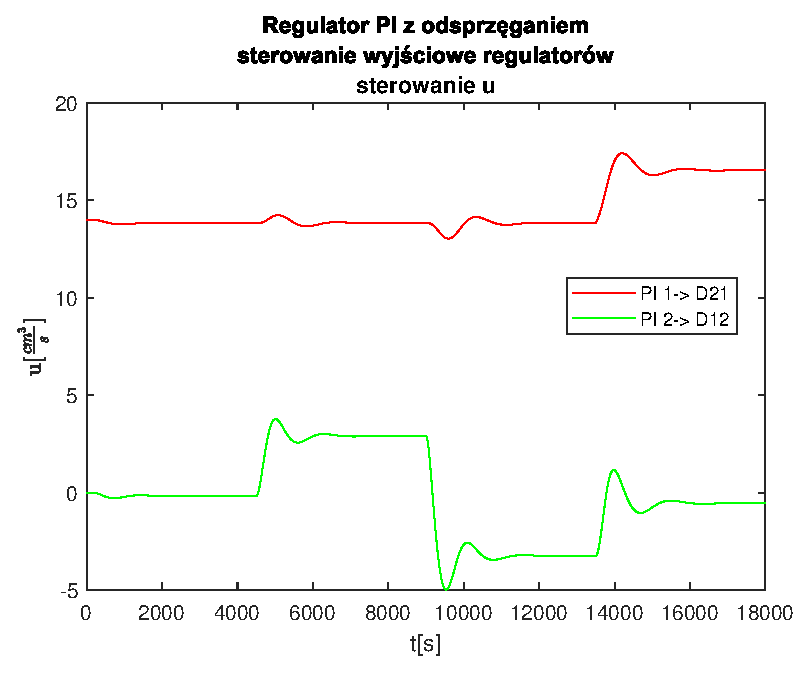
\includegraphics[width=1\linewidth]{img/PI/decoupler/disturbance/PIDecouplerControlD3DisttrueLinfalse.eps}
      \caption{}
      \label{fig:fig:PIDecoupler3DisttrueLinfalse3}
   \end{subfigure}
       
   \begin{subfigure}[b]{0.4\textwidth}
      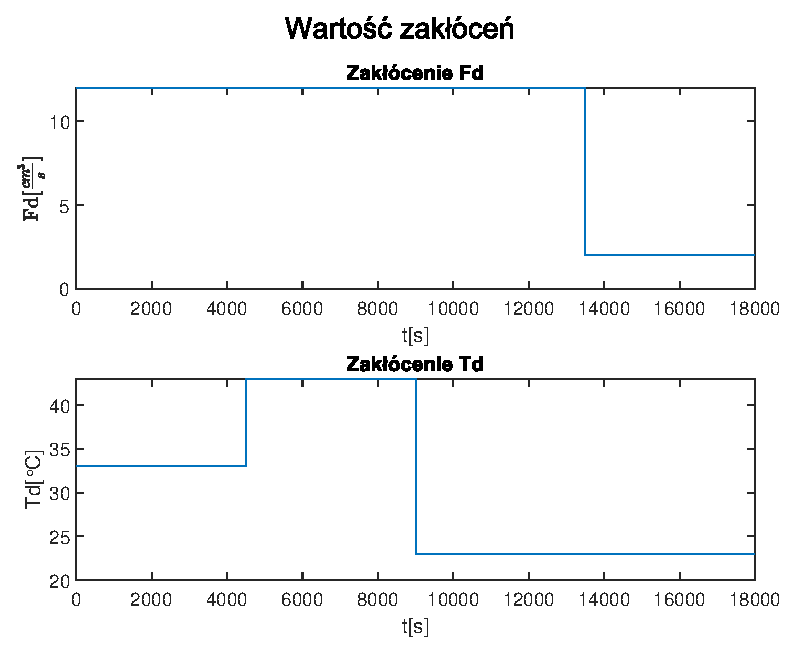
\includegraphics[width=1\linewidth]{img/PI/decoupler/disturbance/PIDecouplerDisturbance3DisttrueLinfalse.eps}
      \caption{}
      \label{fig:fig:PIDecoupler3DisttrueLinfalse4}
   \end{subfigure}
       
   \caption{Wykresy dla regulatora PI z odsprzeganiem dla różnych wartości zakłóceń}
   \label{fig:PIDecoupler3DisttrueLinfalse}
\end{figure}
           

\FloatBarrier


\subsection{PI dla przykładowych przebiegów z obiektem zlinearyzowanym}
\indent Badając jak zachowa się regulator po symulacji na obiekcie zlinearyzowanym widać, że zachowuje się on trochę bardziej stabilnie w wartości skrajnej temperatury zadanej. Jest to zachowanie niebezpieczne, ponieważ wynik z symulacji nie ma przełożenia na rzeczywisty obiekt. Czyli w tym wypadku jest pokazane, że zadana temperaturę można osiągnąć, gdy w rzeczywistości nie jest to możliwe. Należy zatem mieć to na uwadze ograniczenia wynikające z możliwości modelu liniowego.
\FloatBarrier
    \begin{figure}[h!]
   \centering
   \begin{subfigure}[b]{0.4\textwidth}
      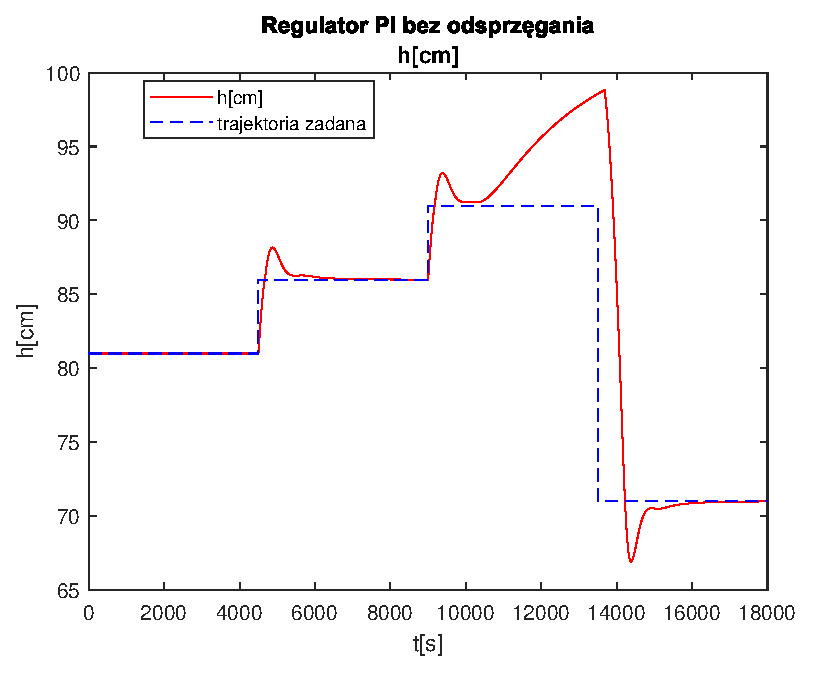
\includegraphics[width=1\linewidth]{img/PI/noDecoupler/noDisturbance/PINoDecouplerH1Lintrue.eps}
      \caption{}
      \label{fig:fig:PINodDecoupler1Lintrue1}
   \end{subfigure}
       
   \begin{subfigure}[b]{0.4\textwidth}
      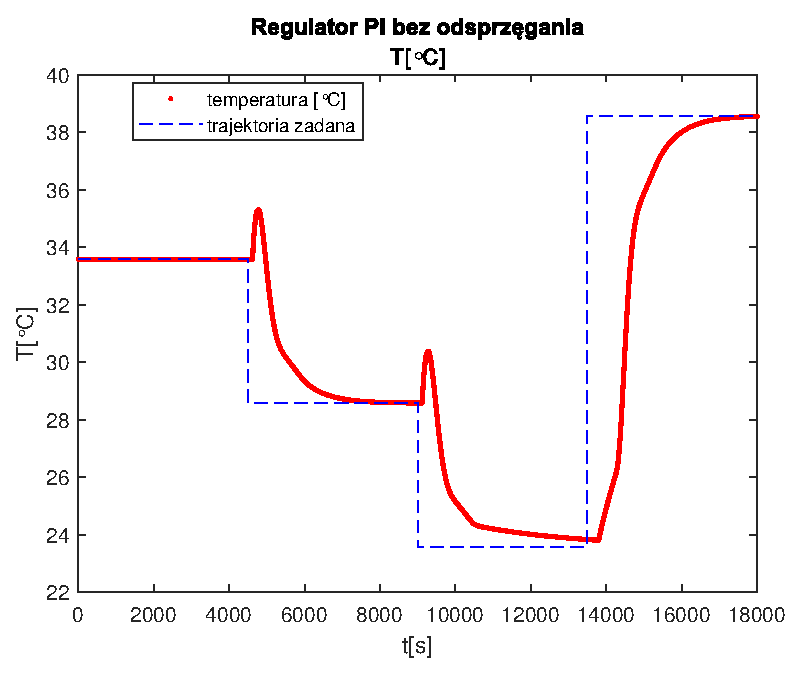
\includegraphics[width=1\linewidth]{img/PI/noDecoupler/noDisturbance/PINoDecouplerT1Lintrue.eps}
      \caption{}
      \label{fig:fig:PINodDecoupler1Lintrue2}
   \end{subfigure}
       
   \begin{subfigure}[b]{0.4\textwidth}
      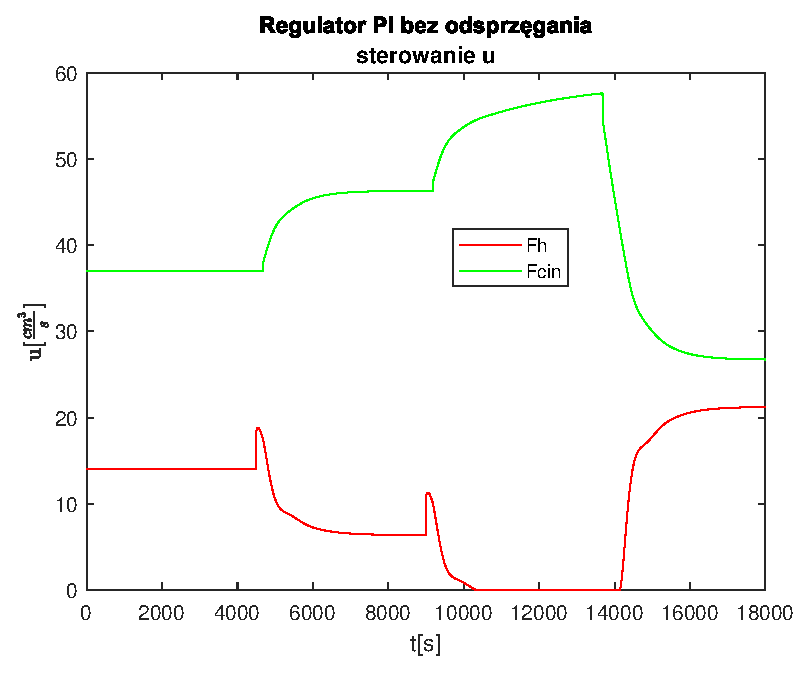
\includegraphics[width=1\linewidth]{img/PI/noDecoupler/noDisturbance/PINoDecouplerControl1Lintrue.eps}
      \caption{}
      \label{fig:fig:PINodDecoupler1Lintrue3}
   \end{subfigure}
       
   \caption{Wykresy dla regulatora PI bez odsprzegania.}
   \label{fig:PINodDecoupler1Lintrue}
\end{figure}
           
\begin{figure}[h!]
   \centering
   \begin{subfigure}[b]{0.4\textwidth}
      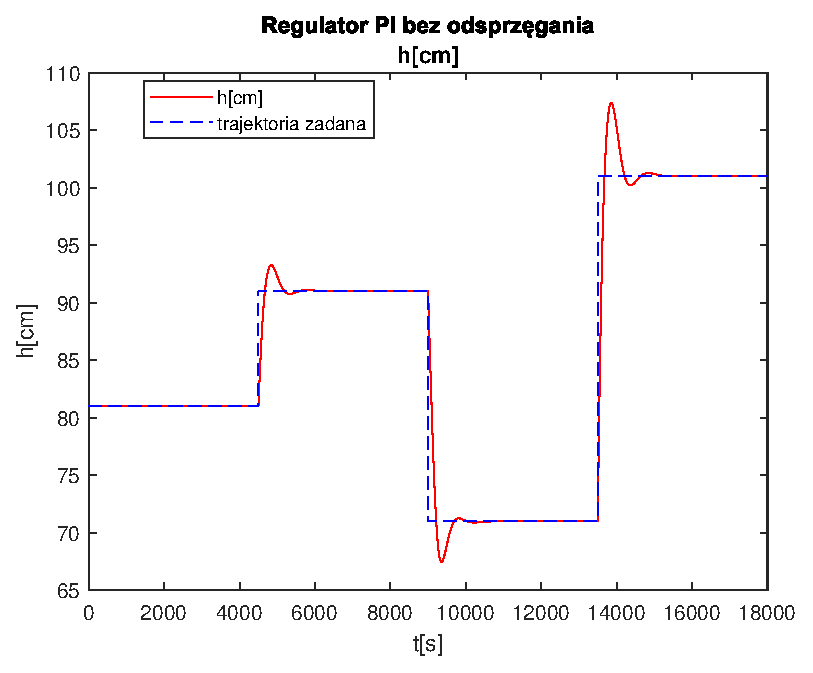
\includegraphics[width=1\linewidth]{img/PI/noDecoupler/noDisturbance/PINoDecouplerH2Lintrue.eps}
      \caption{}
      \label{fig:fig:PINodDecoupler2Lintrue1}
   \end{subfigure}
       
   \begin{subfigure}[b]{0.4\textwidth}
      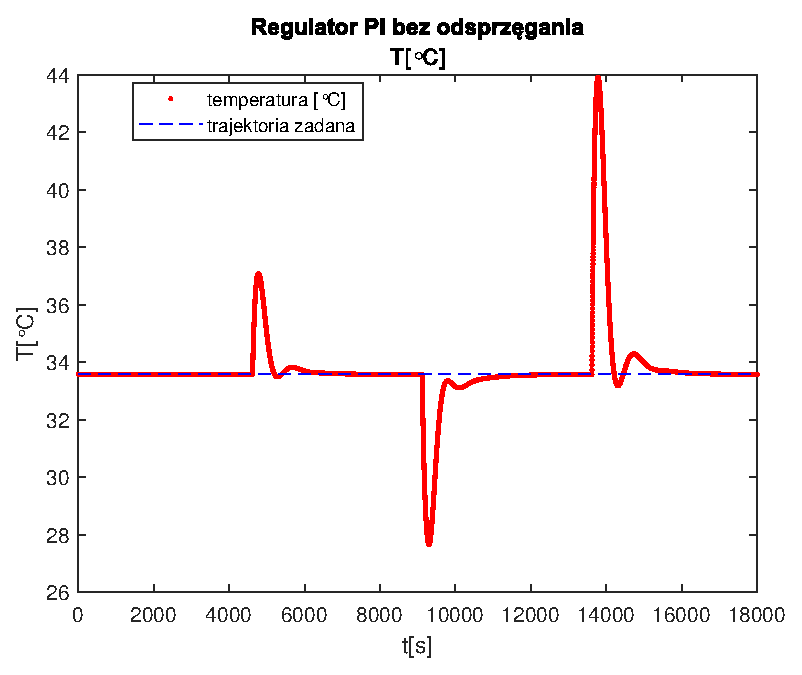
\includegraphics[width=1\linewidth]{img/PI/noDecoupler/noDisturbance/PINoDecouplerT2Lintrue.eps}
      \caption{}
      \label{fig:fig:PINodDecoupler2Lintrue2}
   \end{subfigure}
       
   \begin{subfigure}[b]{0.4\textwidth}
      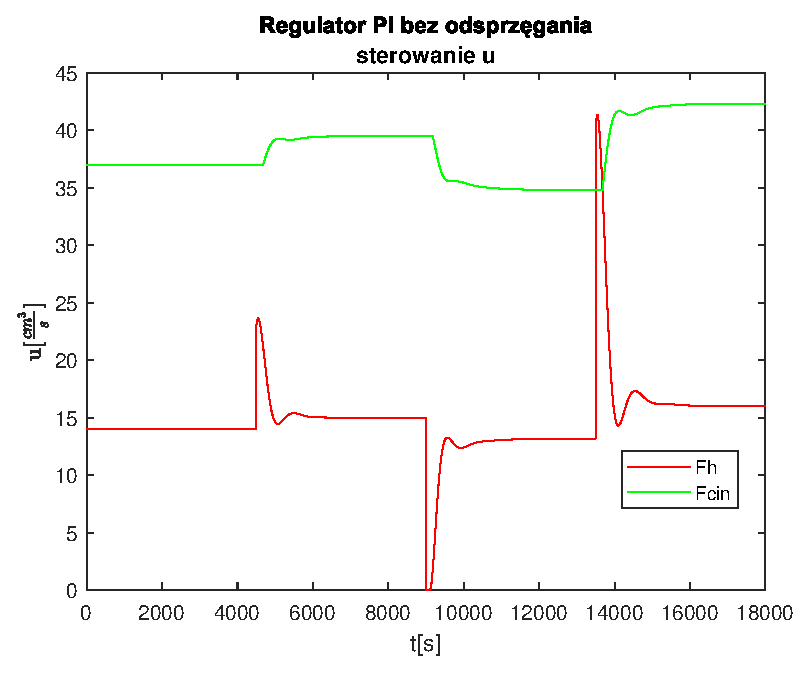
\includegraphics[width=1\linewidth]{img/PI/noDecoupler/noDisturbance/PINoDecouplerControl2Lintrue.eps}
      \caption{}
      \label{fig:fig:PINodDecoupler2Lintrue3}
   \end{subfigure}
       
   \caption{Wykresy dla regulatora PI bez odsprzegania.}
   \label{fig:PINodDecoupler2Lintrue}
\end{figure}
           
\begin{figure}[h!]
   \centering
   \begin{subfigure}[b]{0.4\textwidth}
      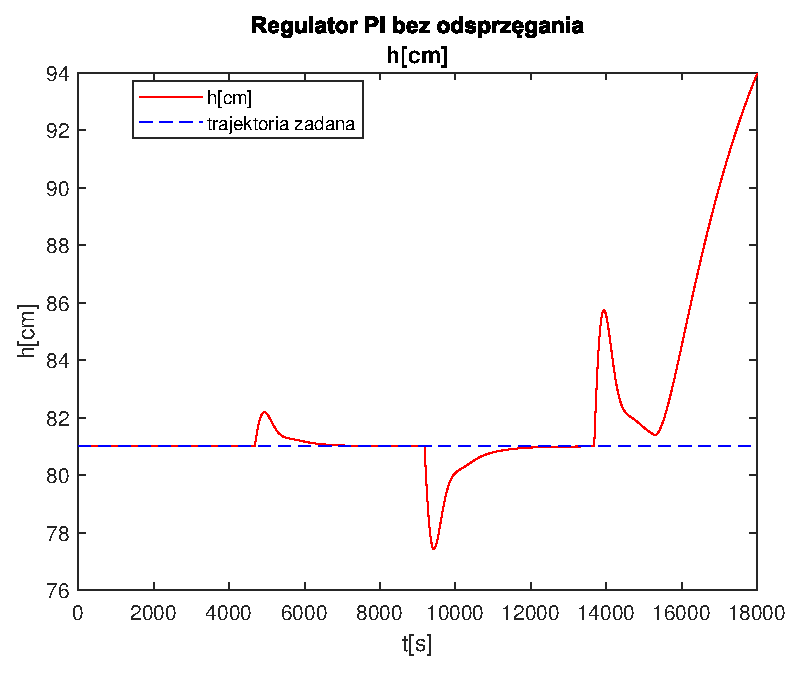
\includegraphics[width=1\linewidth]{img/PI/noDecoupler/noDisturbance/PINoDecouplerH3Lintrue.eps}
      \caption{}
      \label{fig:fig:PINodDecoupler3Lintrue1}
   \end{subfigure}
       
   \begin{subfigure}[b]{0.4\textwidth}
      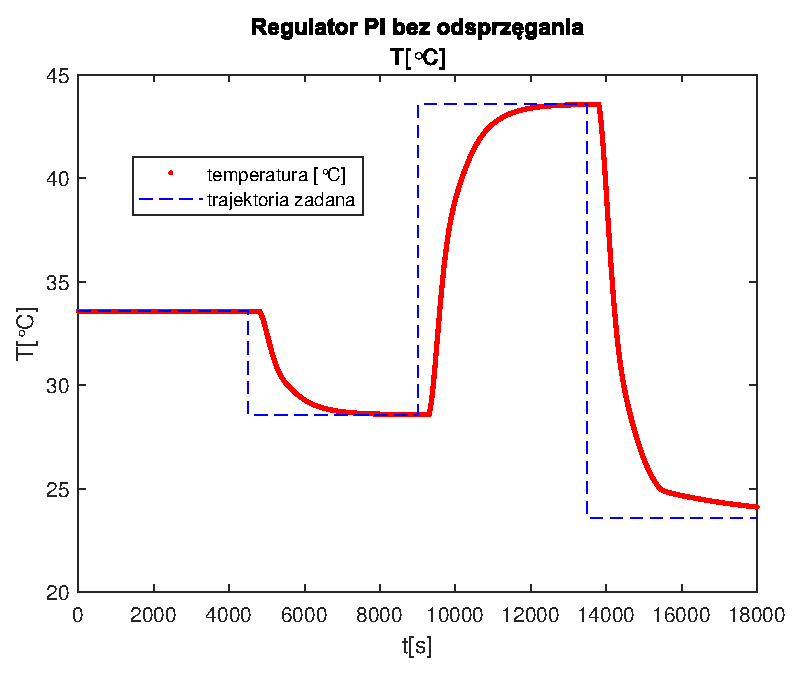
\includegraphics[width=1\linewidth]{img/PI/noDecoupler/noDisturbance/PINoDecouplerT3Lintrue.eps}
      \caption{}
      \label{fig:fig:PINodDecoupler3Lintrue2}
   \end{subfigure}
       
   \begin{subfigure}[b]{0.4\textwidth}
      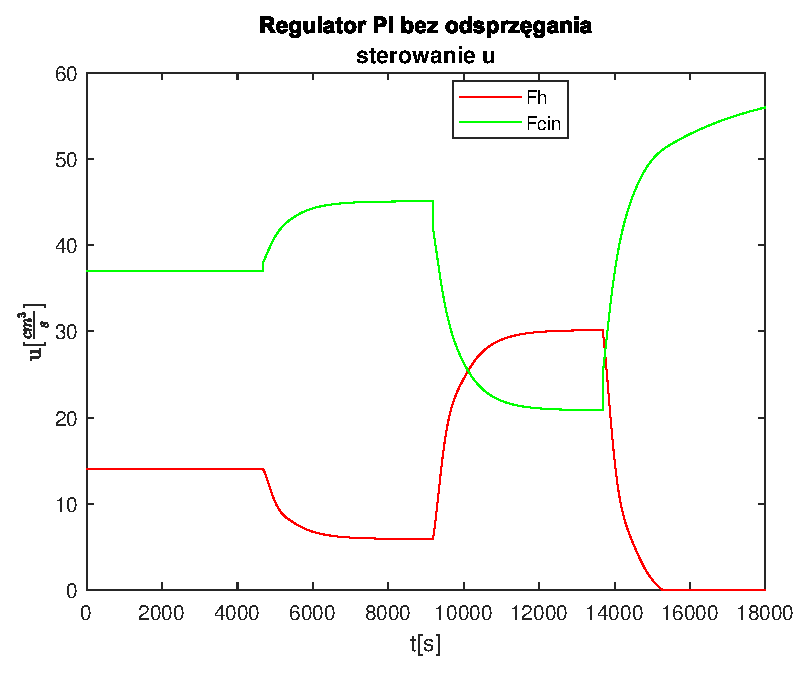
\includegraphics[width=1\linewidth]{img/PI/noDecoupler/noDisturbance/PINoDecouplerControl3Lintrue.eps}
      \caption{}
      \label{fig:fig:PINodDecoupler3Lintrue3}
   \end{subfigure}
       
   \caption{Wykresy dla regulatora PI bez odsprzegania.}
   \label{fig:PINodDecoupler3Lintrue}
\end{figure}
           

\FloatBarrier

\subsection{PI ze zmianą zakłócenia z obiektem nielinowym}
\indent Z wykresów zaprezentowanych w tej sekcji można zaobserwować, że regulator radzi sobie dobrze ze zmianą zakłócenia. Na początku wyjścia odbiegają od wartości zadanych, nie są to jednak są duże wartości. Regulator jest w stanie szybko skompensować zakłócenie i działać potem poprawnie.
\FloatBarrier
    \begin{figure}[h!]
   \centering
   \begin{subfigure}[b]{0.4\textwidth}
      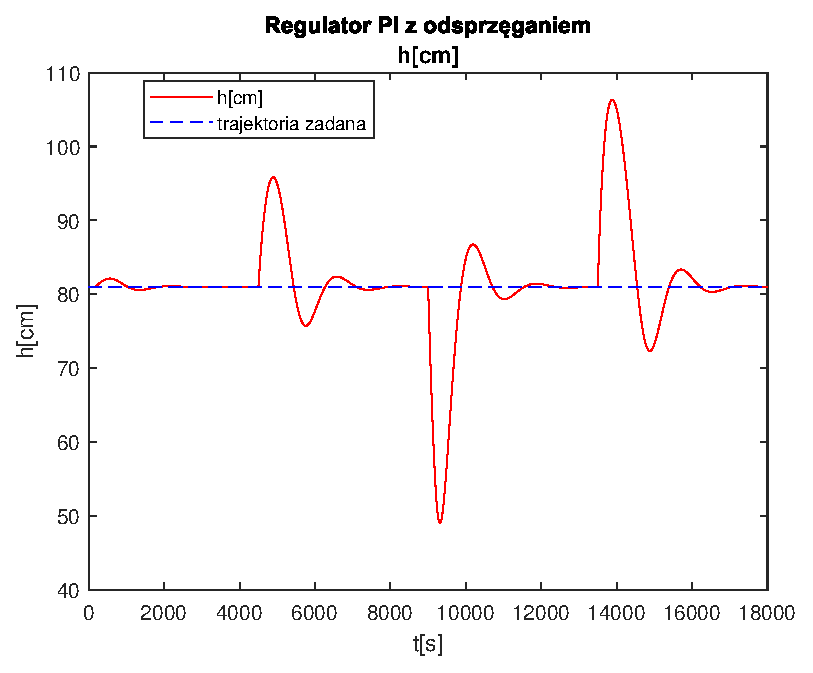
\includegraphics[width=1\linewidth]{img/PI/decoupler/disturbance/PIDecouplerH2DisttrueLinfalse.eps}
      \caption{}
      \label{fig:fig:PIDecoupler2DisttrueLinfalse1}
   \end{subfigure}
       
   \begin{subfigure}[b]{0.4\textwidth}
      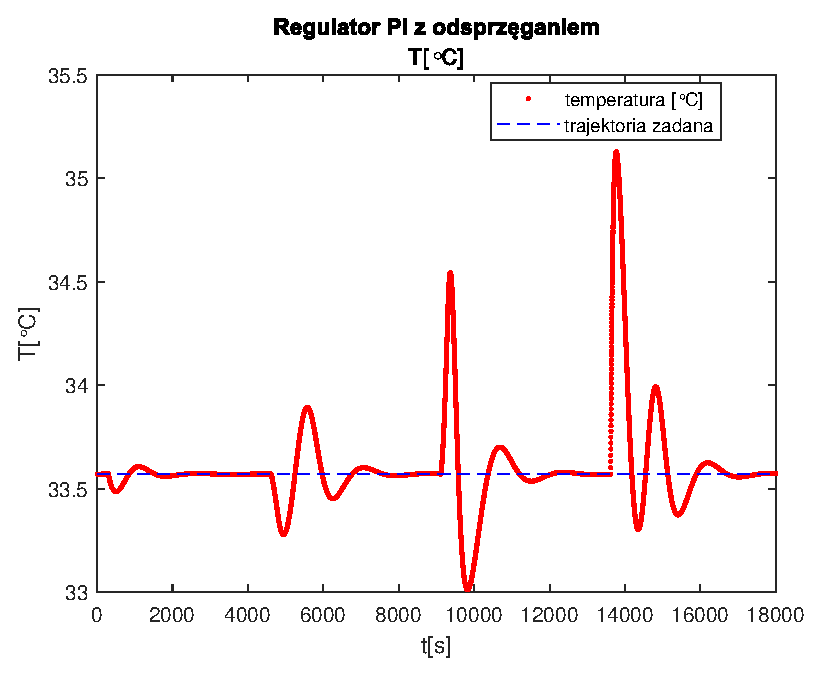
\includegraphics[width=1\linewidth]{img/PI/decoupler/disturbance/PIDecouplerT2DisttrueLinfalse.eps}
      \caption{}
      \label{fig:fig:PIDecoupler2DisttrueLinfalse2}
   \end{subfigure}
       
   \begin{subfigure}[b]{0.4\textwidth}
      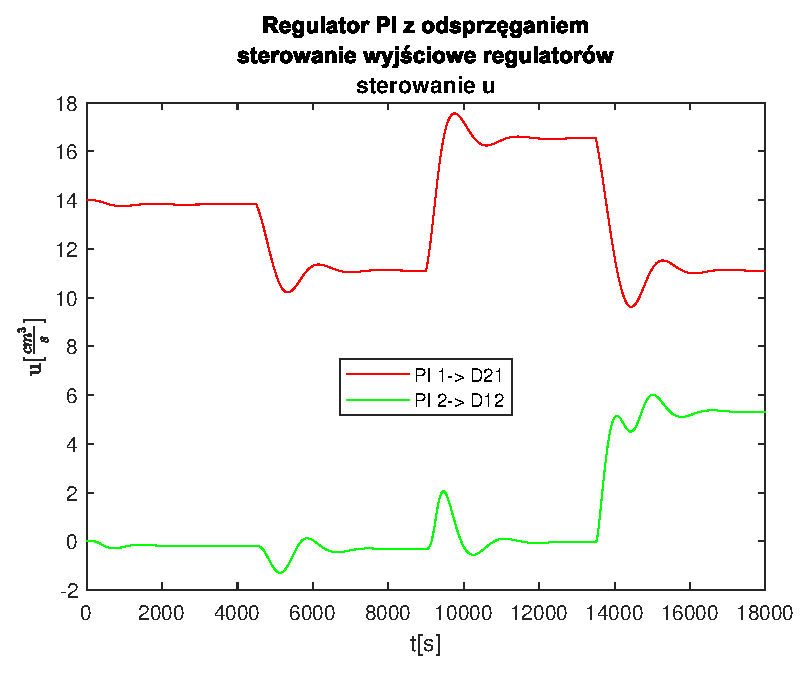
\includegraphics[width=1\linewidth]{img/PI/decoupler/disturbance/PIDecouplerControlD2DisttrueLinfalse.eps}
      \caption{}
      \label{fig:fig:PIDecoupler2DisttrueLinfalse3}
   \end{subfigure}
       
   \begin{subfigure}[b]{0.4\textwidth}
      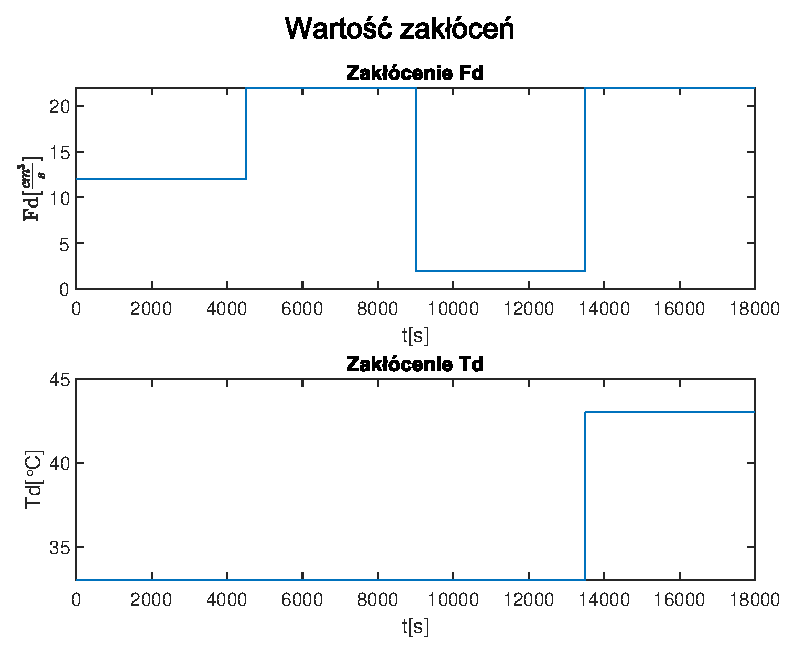
\includegraphics[width=1\linewidth]{img/PI/decoupler/disturbance/PIDecouplerDisturbance2DisttrueLinfalse.eps}
      \caption{}
      \label{fig:fig:PIDecoupler2DisttrueLinfalse4}
   \end{subfigure}
       
   \caption{Wykresy dla regulatora PI z odsprzeganiem dla różnych wartości zakłóceń}
   \label{fig:PIDecoupler2DisttrueLinfalse}
\end{figure}
           
\begin{figure}[h!]
   \centering
   \begin{subfigure}[b]{0.4\textwidth}
      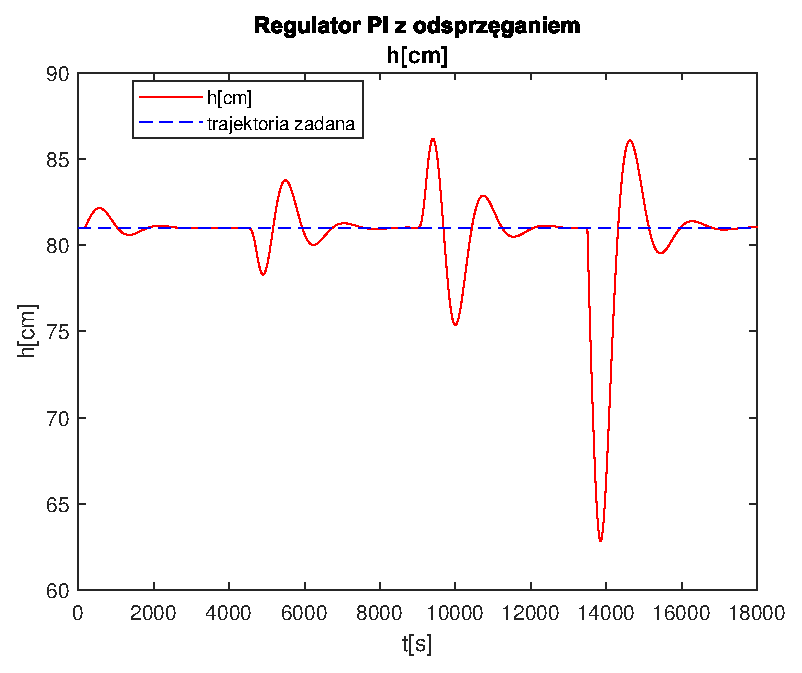
\includegraphics[width=1\linewidth]{img/PI/decoupler/disturbance/PIDecouplerH3DisttrueLinfalse.eps}
      \caption{}
      \label{fig:fig:PIDecoupler3DisttrueLinfalse1}
   \end{subfigure}
       
   \begin{subfigure}[b]{0.4\textwidth}
      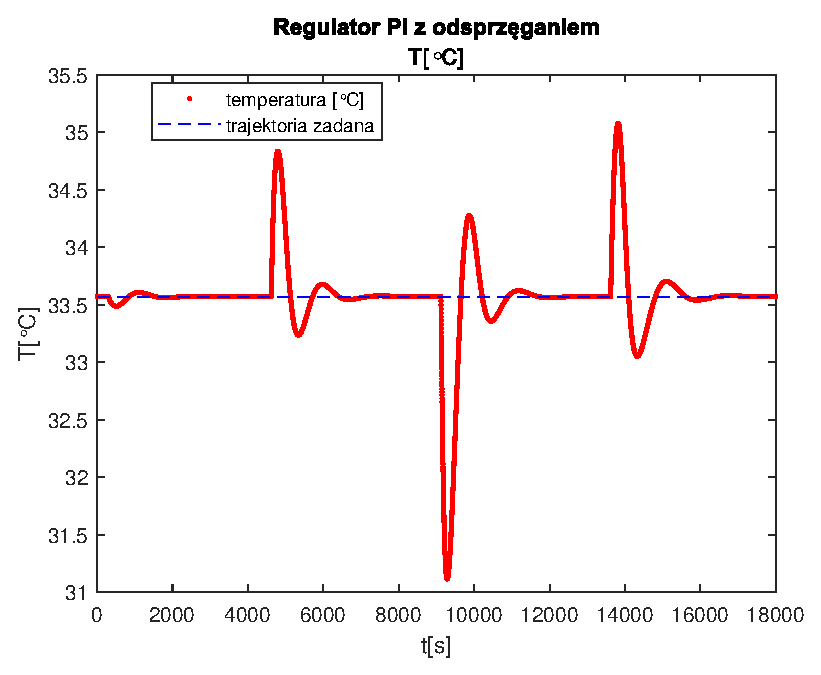
\includegraphics[width=1\linewidth]{img/PI/decoupler/disturbance/PIDecouplerT3DisttrueLinfalse.eps}
      \caption{}
      \label{fig:fig:PIDecoupler3DisttrueLinfalse2}
   \end{subfigure}
       
   \begin{subfigure}[b]{0.4\textwidth}
      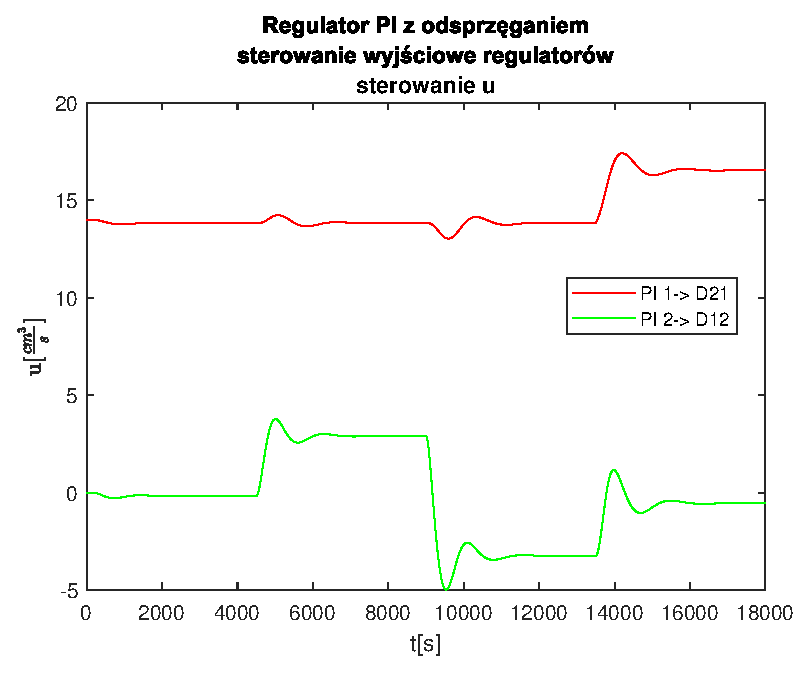
\includegraphics[width=1\linewidth]{img/PI/decoupler/disturbance/PIDecouplerControlD3DisttrueLinfalse.eps}
      \caption{}
      \label{fig:fig:PIDecoupler3DisttrueLinfalse3}
   \end{subfigure}
       
   \begin{subfigure}[b]{0.4\textwidth}
      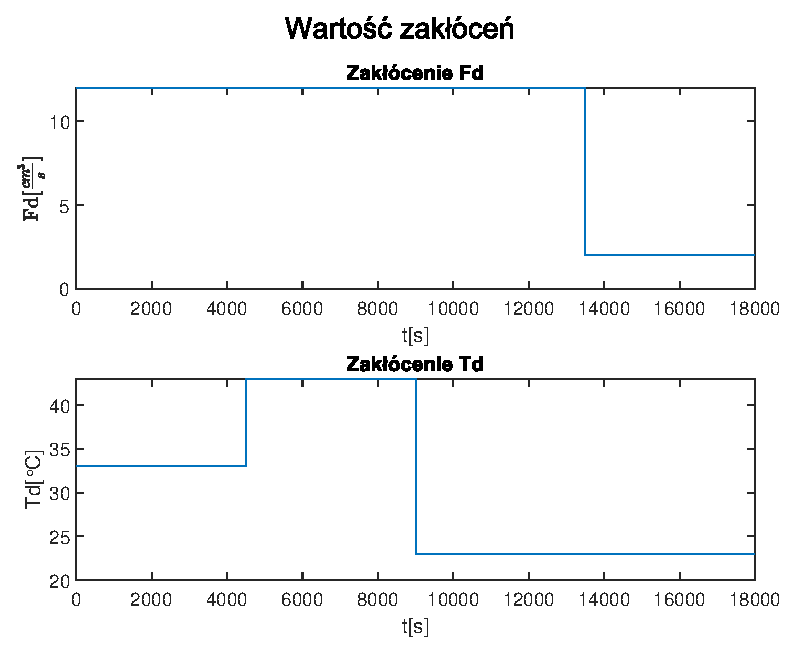
\includegraphics[width=1\linewidth]{img/PI/decoupler/disturbance/PIDecouplerDisturbance3DisttrueLinfalse.eps}
      \caption{}
      \label{fig:fig:PIDecoupler3DisttrueLinfalse4}
   \end{subfigure}
       
   \caption{Wykresy dla regulatora PI z odsprzeganiem dla różnych wartości zakłóceń}
   \label{fig:PIDecoupler3DisttrueLinfalse}
\end{figure}
           

\FloatBarrier


\subsection{Napełniania zbiornika do punktu pracy PI z modelem nieliniowym}
\indent W ramach testów zostało sprawdzone jak regulator radzi sobie z zapełnianiem zbiornika. W związku z tym, że sterownie dojścia zimnej wody jest opóźnione występuje znaczące przergulowanie temperatury, ponieważ głównie to regulator odpowiadający za dopływ ciepłej wody odpowiada za strumień wejściowy. Dzieje się tak ponieważ temperatura zadana jest wyższa niż obecna w zbiorniku oraz że zimna woda działa z opóźnieniem. Po chwili gdy wejście zimnej wody również zaczyna mieć wpływ w obiekcie układ się stabilizuje.
\FloatBarrier
    \begin{figure}[h!]
   \centering
   \begin{subfigure}[b]{0.4\textwidth}
      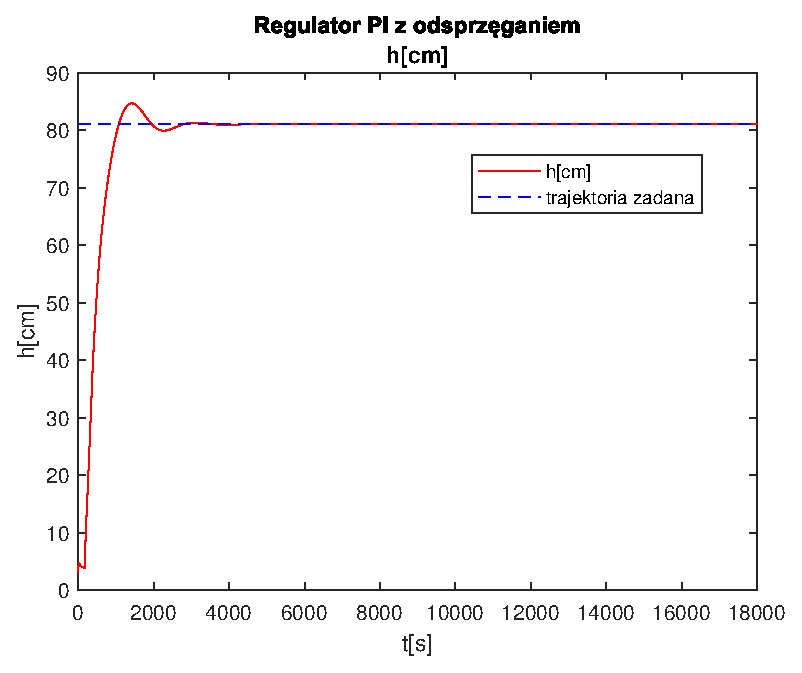
\includegraphics[width=1\linewidth]{img/PI/decoupler/noDisturbance/PIDecouplerH0.eps}
      \caption{}
      \label{fig:fig:PIDecoupler01}
   \end{subfigure}
       
   \begin{subfigure}[b]{0.4\textwidth}
      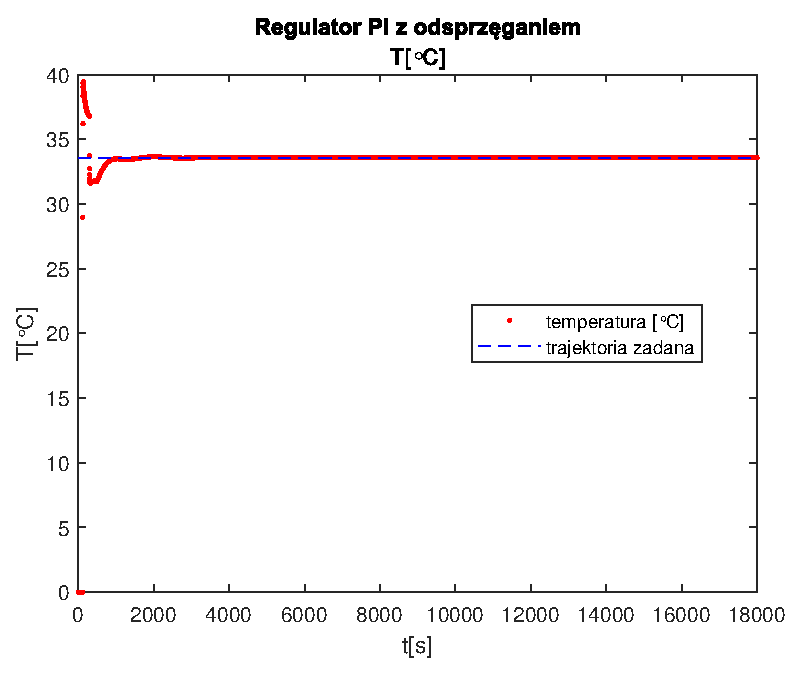
\includegraphics[width=1\linewidth]{img/PI/decoupler/noDisturbance/PIDecouplerT0.eps}
      \caption{}
      \label{fig:fig:PIDecoupler02}
   \end{subfigure}
       
   \begin{subfigure}[b]{0.4\textwidth}
      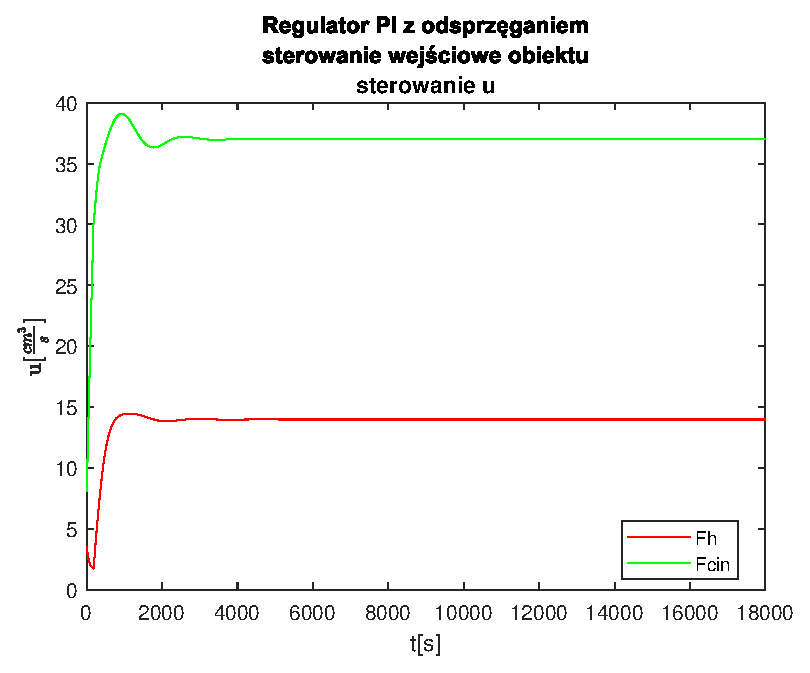
\includegraphics[width=1\linewidth]{img/PI/decoupler/noDisturbance/PIDecouplerControl0.eps}
      \caption{}
      \label{fig:fig:PIDecoupler03}
   \end{subfigure}
       
   \begin{subfigure}[b]{0.4\textwidth}
      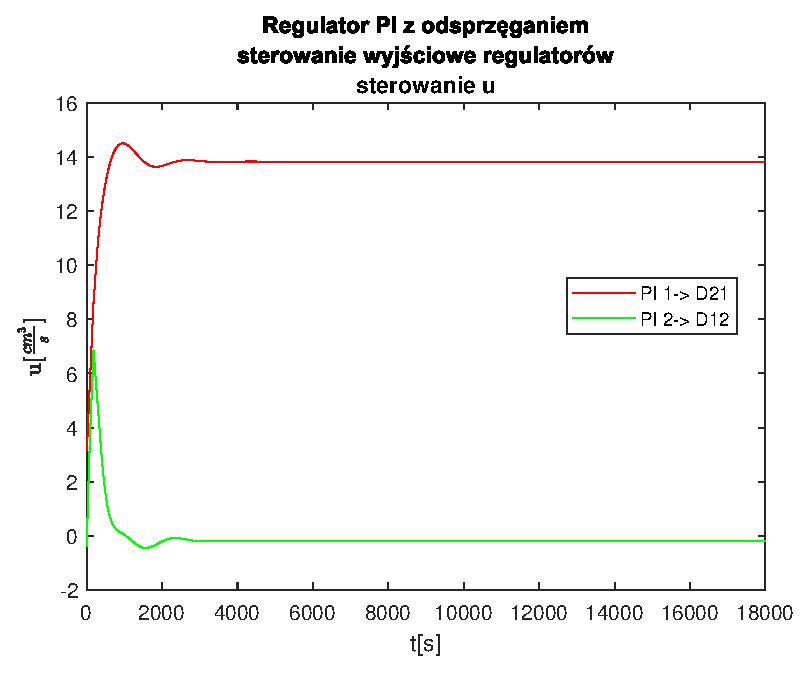
\includegraphics[width=1\linewidth]{img/PI/decoupler/noDisturbance/PIDecouplerControlD0.eps}
      \caption{}
      \label{fig:fig:PIDecoupler04}
   \end{subfigure}
       
   \caption{Wykresy dla regulatora PI z odsprzeganiem.}
   \label{fig:PIDecoupler0}
\end{figure}
           

\FloatBarrier 
\newpage
\section{Regulator PI z odsprzęganiem}
\indent Pierwszy otrzymany regulator z odsprzęganiem działał dużo gorzej od regulatora PID. Wynikało, to głownie z faktu, że bloki odsprzęgające są jak niżej zaprezentowano elementem liniowym lub w przybliżeniu linowym (czyli ich stosunek tez był liniowy, gdy jedna z wartości osiągała wartość 0). Toteż gdy sygnały z regulatorów były przycinane tak jak dla regulatora bez odsprzęgania regulator nie był w stanie osiągnąć temperatury wyższej niż w punkcie pracy. Rozwiązaniem tego problemu było wprowadzenie ograniczenia ujemnego dla sygnałów wyjściowych z regulatora i wprowadzenie minimalnej wartości sygnalu sterowania 0 dopiero po z sumowaniu sygnału z regulatora z sygnałem z bloku odsprzęgającego. Po tym zabiegu widać czasem pozytywny wpływ bloku odsprzęgającego na jakość regulacji.

\indent Człony odsprzęgające prezentują się następującymi równaniami:\\
\begin{equation}
    D12=-1
\end{equation}
\begin{equation}
    D21=\frac{0.00619z+2.122e-5}{0.002301z+7.897e-6}=~2.69
\end{equation}

\indent Transmitancja $D21$ sprowadza się do równania różnicowego:
\begin{equation}
    y(k)=\frac{7.897e-6y(k-1)+0.00619u(k)++2.122e-5u(k-1)}{0.002301}
\end{equation}

 W przypadku członu odsprzęgającego $D21$ zbadano zarówno odsprzęganie w przybliżonej formie  po wyzerowaniu składowych bliskich zeru) jak i wyrażone za pomocą równania różnicowego. Różnice były niezauważalne, na wykresach zostały przedstawione regulatory przy użyciu bardziej zaawansowanej formy.

\subsection{Dobrane nastawy regulatora PI}
\indent Parametry regulatora zostały dobrane w ten sam sposób co dla regulatora bez odsprzęgania. Również zostały zastosowane takie same ograniczenia na maksymalną wartość na maksymalną wartość sterowania oraz ten sam algorytm anti-windup. Minimalna wartość sterowania jest równa maksymalnej maksymalnej pomnożonej przez minus jeden. Przycinanie sygnałów jest również zrealizowana na wyjściu członów odsprzęgających.\\
\indent Dobrane parametry są następujące: \\
$KpFh=0.04$   $KiFh= 0.0004$ \\
$KpFcin= 0$  $ KiFcin2=-0.01$ \\



\subsection{PI dla przykładowych przebiegów z obiektem nielinowym}
\indent Największą zaletą jaką widać po wprowadzeniu bloku odsprzegania jest fakt, że uklad jest bardziej odporny na zadanie wartości skrajnej, jak w tym wypadku temperatury bliskiej minimalnej. Regulator już nie próbuję usunąć uchybu ustalonego i układ się stabilizuje.  \\
\indent Negatywnym zjawiskiem jest przypadek gdy wysokość słupa cieczy dąży do zera dla jednoczesnego wzrostu temperatury zadanej i zmniejszenia wysokości zadanej. Wynika to z faktu, że regulator próbuje zmniejszyć wysokosć słupa cieczy, ale przez odsprzęganie wyłącza oba dopływy.
% \FloatBarrier
%     \begin{figure}[h!]
   \centering
   \begin{subfigure}[b]{0.4\textwidth}
      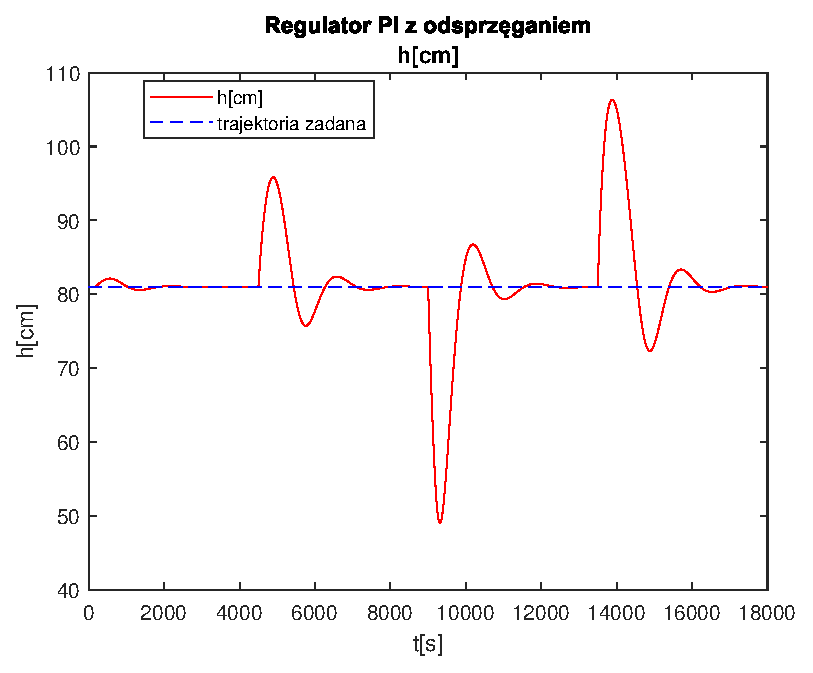
\includegraphics[width=1\linewidth]{img/PI/decoupler/disturbance/PIDecouplerH2DisttrueLinfalse.eps}
      \caption{}
      \label{fig:fig:PIDecoupler2DisttrueLinfalse1}
   \end{subfigure}
       
   \begin{subfigure}[b]{0.4\textwidth}
      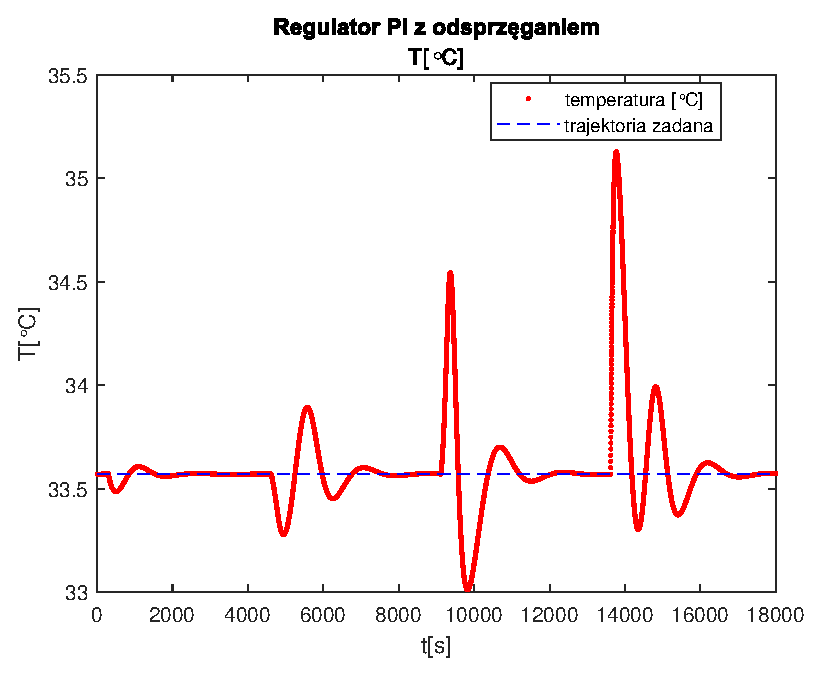
\includegraphics[width=1\linewidth]{img/PI/decoupler/disturbance/PIDecouplerT2DisttrueLinfalse.eps}
      \caption{}
      \label{fig:fig:PIDecoupler2DisttrueLinfalse2}
   \end{subfigure}
       
   \begin{subfigure}[b]{0.4\textwidth}
      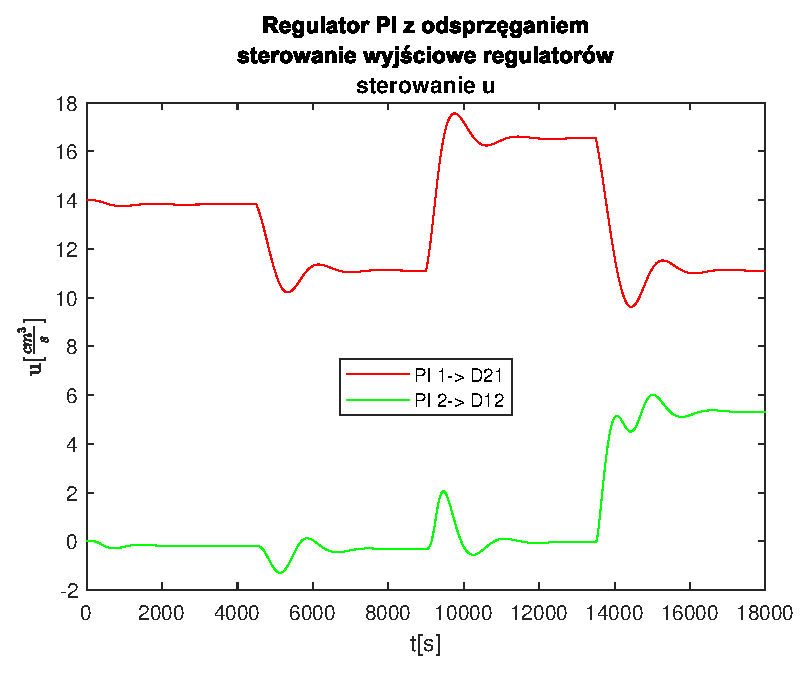
\includegraphics[width=1\linewidth]{img/PI/decoupler/disturbance/PIDecouplerControlD2DisttrueLinfalse.eps}
      \caption{}
      \label{fig:fig:PIDecoupler2DisttrueLinfalse3}
   \end{subfigure}
       
   \begin{subfigure}[b]{0.4\textwidth}
      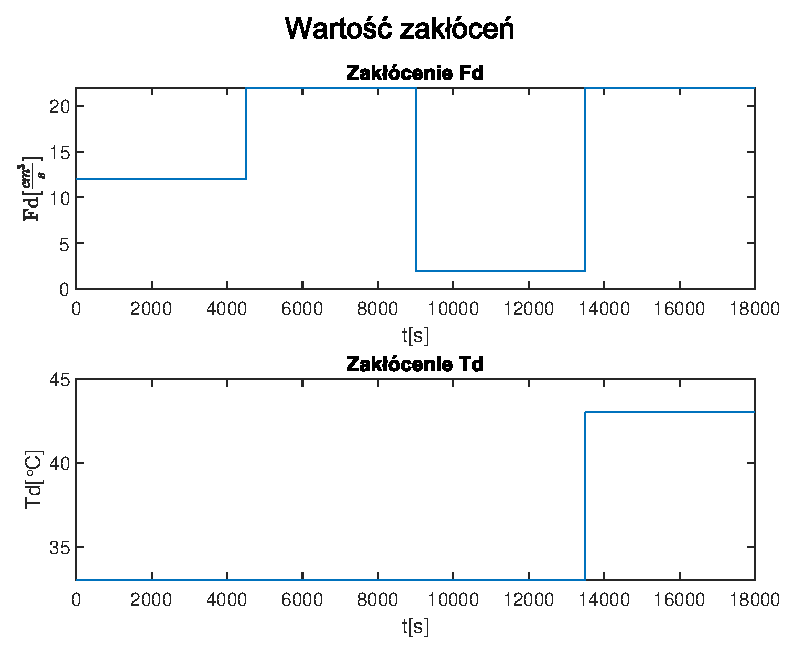
\includegraphics[width=1\linewidth]{img/PI/decoupler/disturbance/PIDecouplerDisturbance2DisttrueLinfalse.eps}
      \caption{}
      \label{fig:fig:PIDecoupler2DisttrueLinfalse4}
   \end{subfigure}
       
   \caption{Wykresy dla regulatora PI z odsprzeganiem dla różnych wartości zakłóceń}
   \label{fig:PIDecoupler2DisttrueLinfalse}
\end{figure}
           
\begin{figure}[h!]
   \centering
   \begin{subfigure}[b]{0.4\textwidth}
      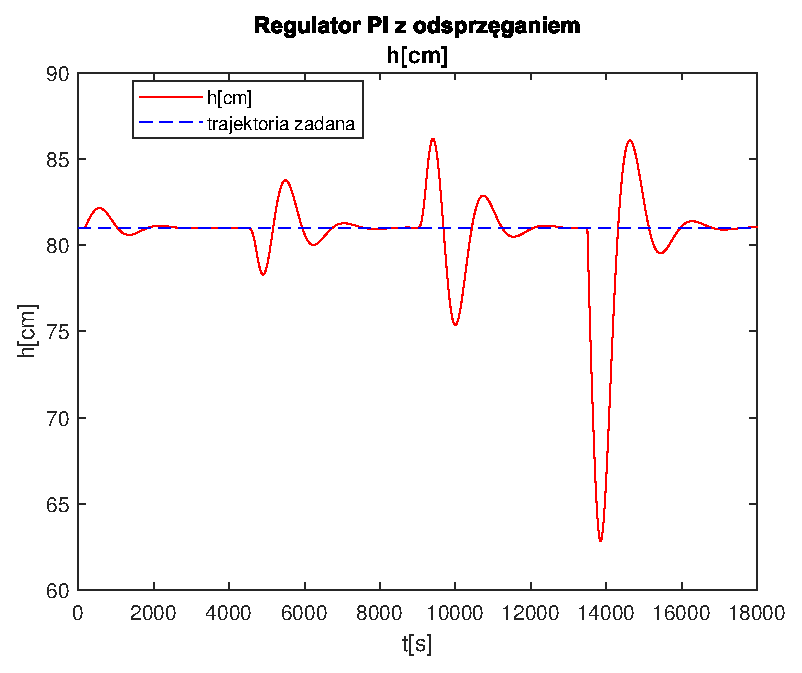
\includegraphics[width=1\linewidth]{img/PI/decoupler/disturbance/PIDecouplerH3DisttrueLinfalse.eps}
      \caption{}
      \label{fig:fig:PIDecoupler3DisttrueLinfalse1}
   \end{subfigure}
       
   \begin{subfigure}[b]{0.4\textwidth}
      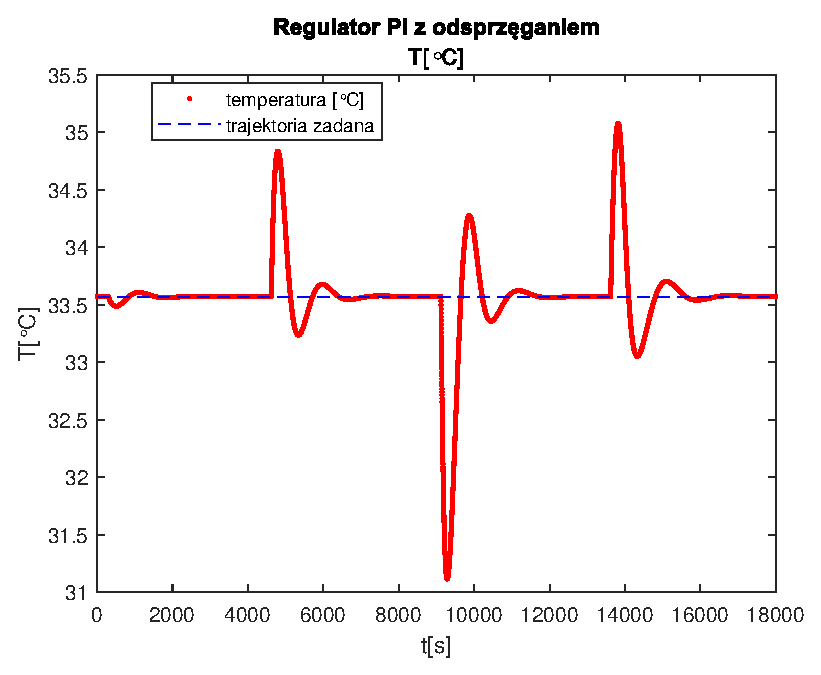
\includegraphics[width=1\linewidth]{img/PI/decoupler/disturbance/PIDecouplerT3DisttrueLinfalse.eps}
      \caption{}
      \label{fig:fig:PIDecoupler3DisttrueLinfalse2}
   \end{subfigure}
       
   \begin{subfigure}[b]{0.4\textwidth}
      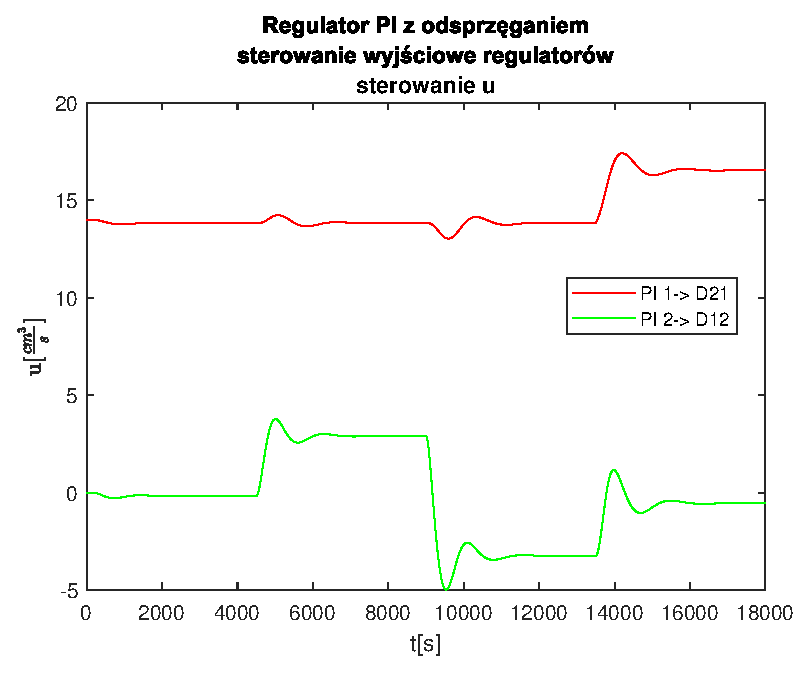
\includegraphics[width=1\linewidth]{img/PI/decoupler/disturbance/PIDecouplerControlD3DisttrueLinfalse.eps}
      \caption{}
      \label{fig:fig:PIDecoupler3DisttrueLinfalse3}
   \end{subfigure}
       
   \begin{subfigure}[b]{0.4\textwidth}
      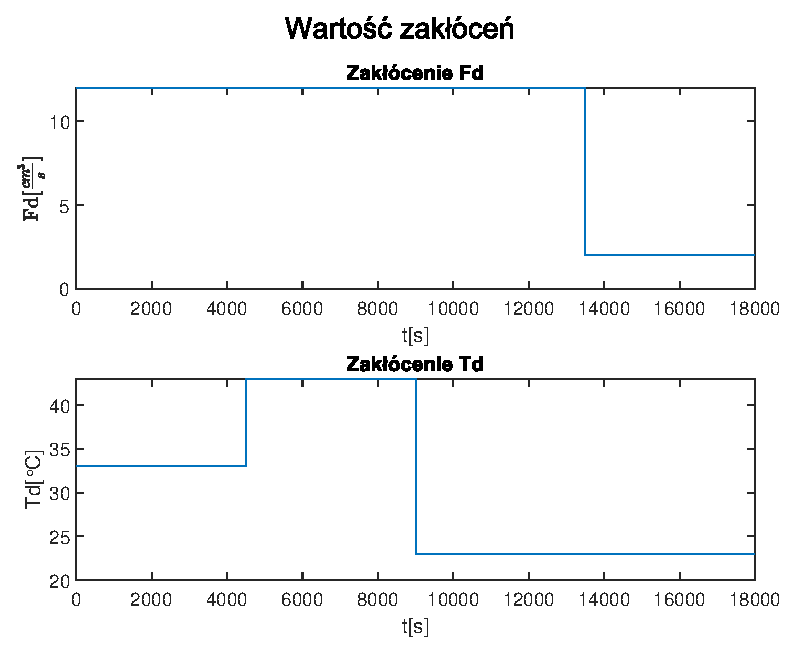
\includegraphics[width=1\linewidth]{img/PI/decoupler/disturbance/PIDecouplerDisturbance3DisttrueLinfalse.eps}
      \caption{}
      \label{fig:fig:PIDecoupler3DisttrueLinfalse4}
   \end{subfigure}
       
   \caption{Wykresy dla regulatora PI z odsprzeganiem dla różnych wartości zakłóceń}
   \label{fig:PIDecoupler3DisttrueLinfalse}
\end{figure}
           

% \FloatBarrier


\subsection{PI dla przykładowych przebiegów z obiektem zlinearyzowanym}
\indent Zostało również zbadane jak będzie się zachowywała sie symulacja gdy sterowania podamy na model zlinearyzowany. W tym wypadku zastosowanie modelu zlinearyzowanego do symulacji jest jeszcze bardziej niebezpieczne, ponieważ można osiągnąć wartość minimalną mniejszą niż jest w ogóle możliwa (temperatura mniejsza  jest od Tc w przypadku przergulowania).
\FloatBarrier
    \begin{figure}[h!]
   \centering
   \begin{subfigure}[b]{0.4\textwidth}
      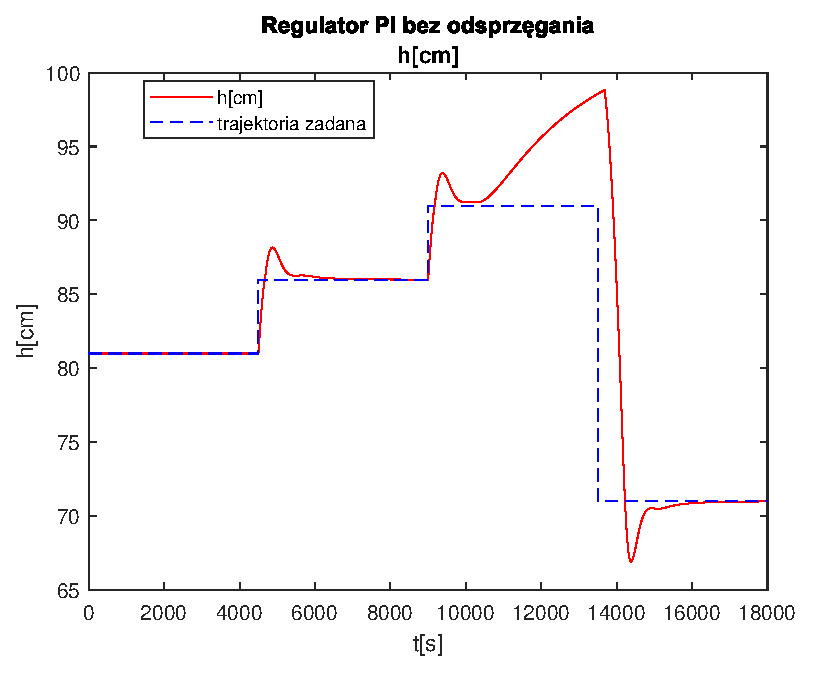
\includegraphics[width=1\linewidth]{img/PI/noDecoupler/noDisturbance/PINoDecouplerH1Lintrue.eps}
      \caption{}
      \label{fig:fig:PINodDecoupler1Lintrue1}
   \end{subfigure}
       
   \begin{subfigure}[b]{0.4\textwidth}
      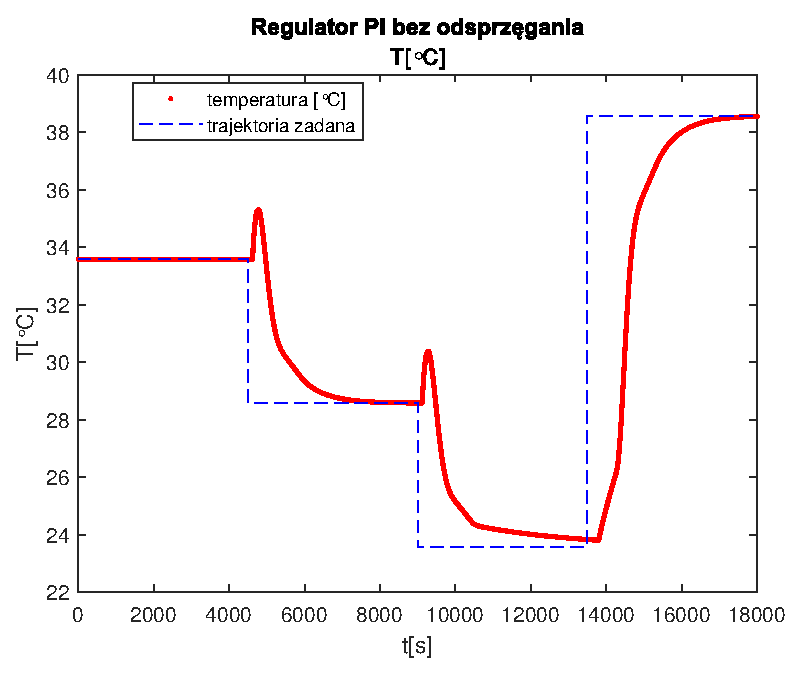
\includegraphics[width=1\linewidth]{img/PI/noDecoupler/noDisturbance/PINoDecouplerT1Lintrue.eps}
      \caption{}
      \label{fig:fig:PINodDecoupler1Lintrue2}
   \end{subfigure}
       
   \begin{subfigure}[b]{0.4\textwidth}
      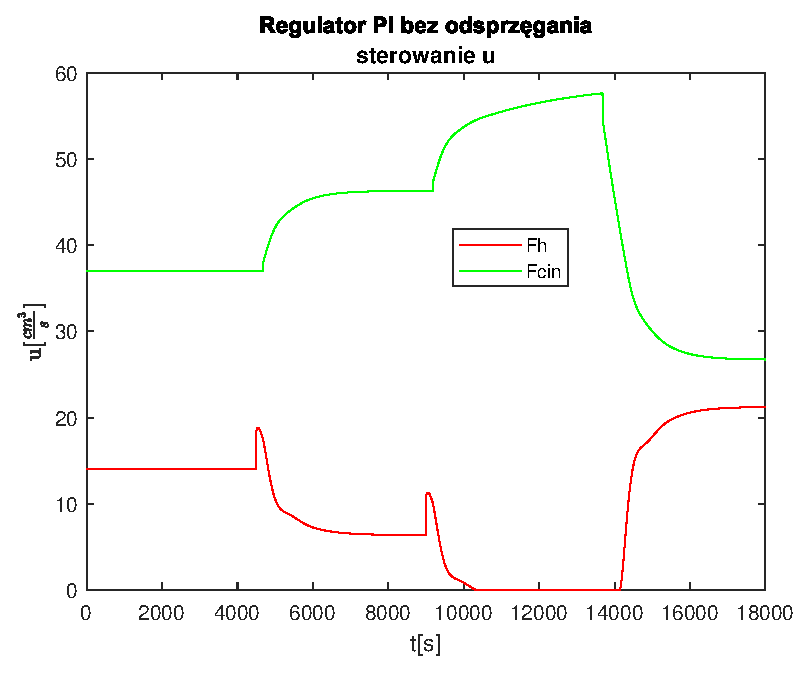
\includegraphics[width=1\linewidth]{img/PI/noDecoupler/noDisturbance/PINoDecouplerControl1Lintrue.eps}
      \caption{}
      \label{fig:fig:PINodDecoupler1Lintrue3}
   \end{subfigure}
       
   \caption{Wykresy dla regulatora PI bez odsprzegania.}
   \label{fig:PINodDecoupler1Lintrue}
\end{figure}
           
\begin{figure}[h!]
   \centering
   \begin{subfigure}[b]{0.4\textwidth}
      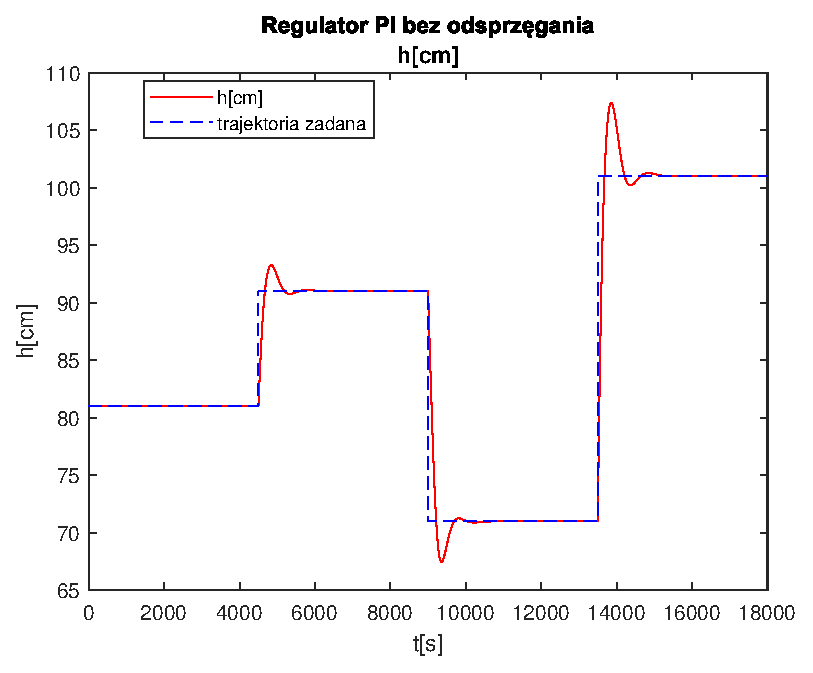
\includegraphics[width=1\linewidth]{img/PI/noDecoupler/noDisturbance/PINoDecouplerH2Lintrue.eps}
      \caption{}
      \label{fig:fig:PINodDecoupler2Lintrue1}
   \end{subfigure}
       
   \begin{subfigure}[b]{0.4\textwidth}
      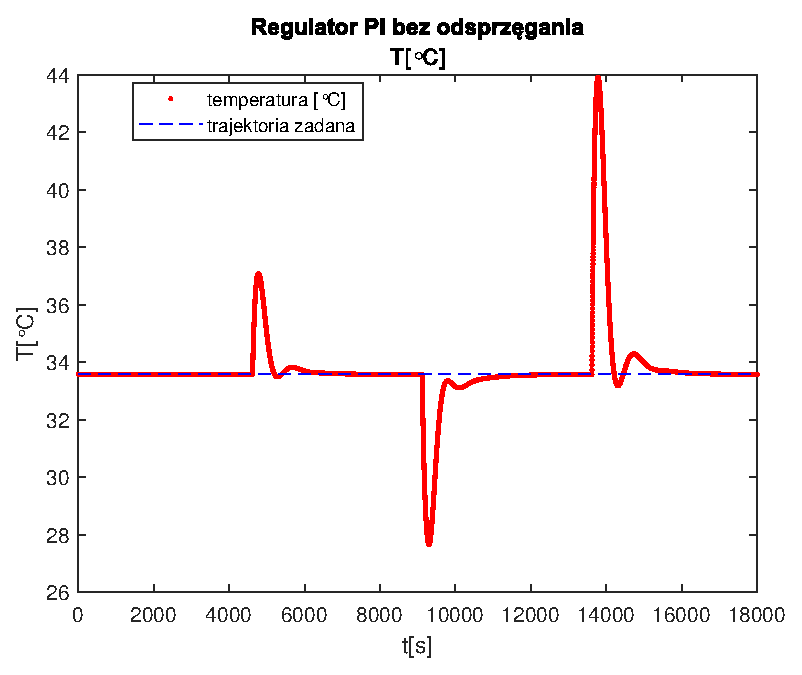
\includegraphics[width=1\linewidth]{img/PI/noDecoupler/noDisturbance/PINoDecouplerT2Lintrue.eps}
      \caption{}
      \label{fig:fig:PINodDecoupler2Lintrue2}
   \end{subfigure}
       
   \begin{subfigure}[b]{0.4\textwidth}
      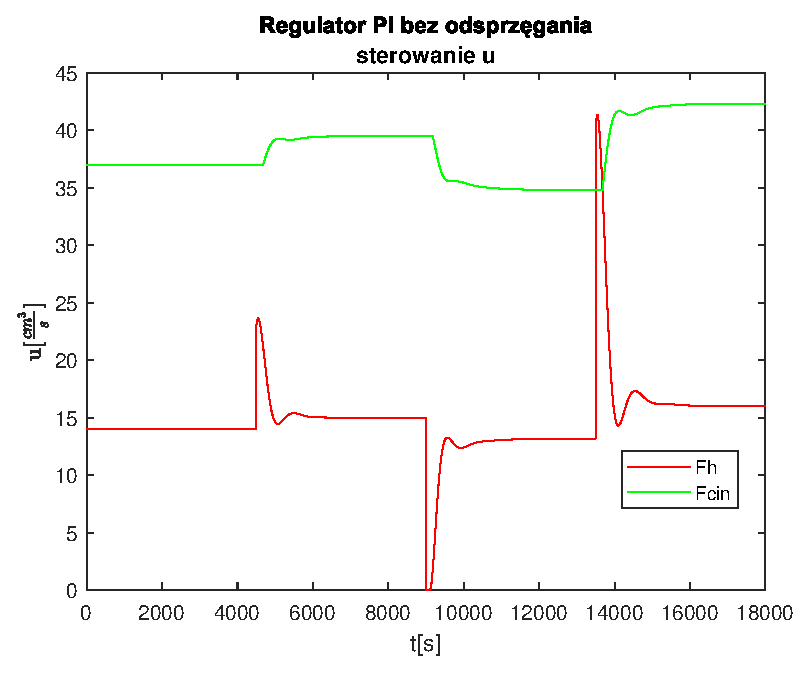
\includegraphics[width=1\linewidth]{img/PI/noDecoupler/noDisturbance/PINoDecouplerControl2Lintrue.eps}
      \caption{}
      \label{fig:fig:PINodDecoupler2Lintrue3}
   \end{subfigure}
       
   \caption{Wykresy dla regulatora PI bez odsprzegania.}
   \label{fig:PINodDecoupler2Lintrue}
\end{figure}
           
\begin{figure}[h!]
   \centering
   \begin{subfigure}[b]{0.4\textwidth}
      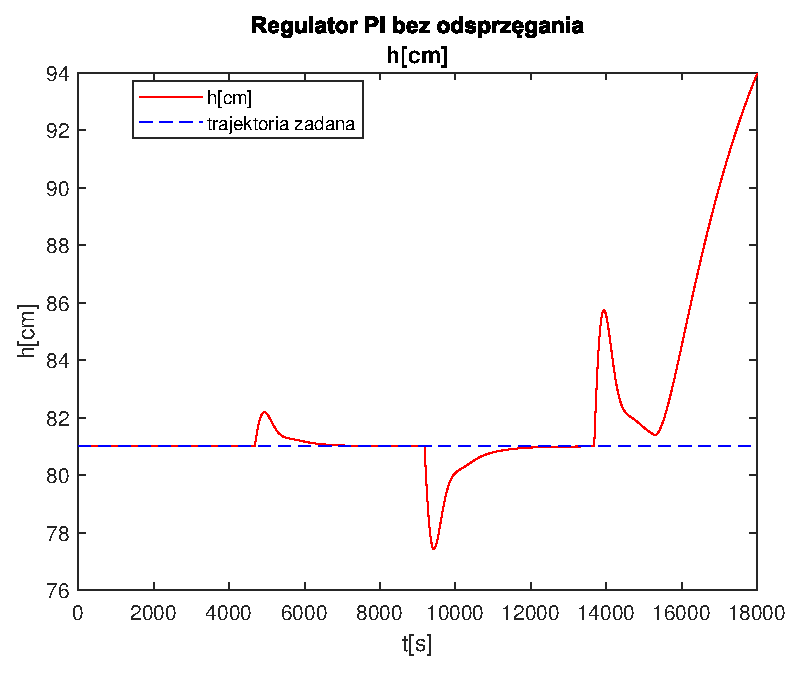
\includegraphics[width=1\linewidth]{img/PI/noDecoupler/noDisturbance/PINoDecouplerH3Lintrue.eps}
      \caption{}
      \label{fig:fig:PINodDecoupler3Lintrue1}
   \end{subfigure}
       
   \begin{subfigure}[b]{0.4\textwidth}
      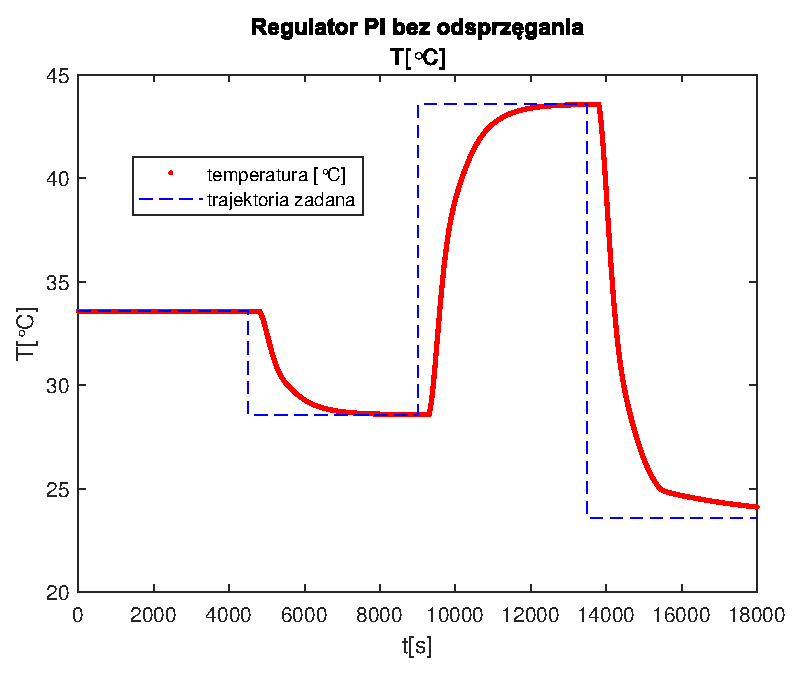
\includegraphics[width=1\linewidth]{img/PI/noDecoupler/noDisturbance/PINoDecouplerT3Lintrue.eps}
      \caption{}
      \label{fig:fig:PINodDecoupler3Lintrue2}
   \end{subfigure}
       
   \begin{subfigure}[b]{0.4\textwidth}
      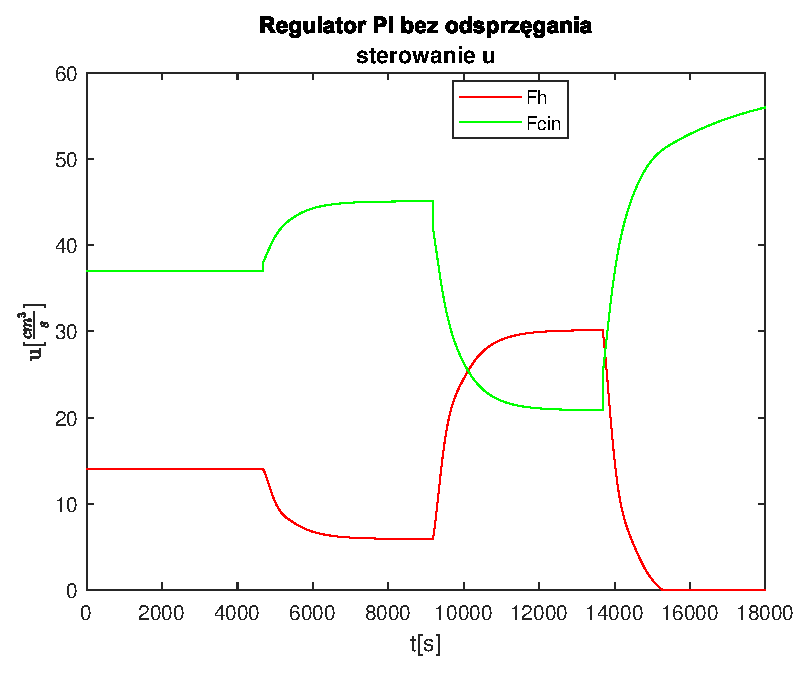
\includegraphics[width=1\linewidth]{img/PI/noDecoupler/noDisturbance/PINoDecouplerControl3Lintrue.eps}
      \caption{}
      \label{fig:fig:PINodDecoupler3Lintrue3}
   \end{subfigure}
       
   \caption{Wykresy dla regulatora PI bez odsprzegania.}
   \label{fig:PINodDecoupler3Lintrue}
\end{figure}
           

\FloatBarrier


\subsection{PI ze zmianą zakłócenia z obiektem nielinowym}
\indent Regulator radzi sobie porównywalnie z regulatorem bez odsprzęgania gdy są podane zakłócenia. Miejscami uchyby są mniejsze lub wprost minimalne. Są jednak przypadki gdy wartości uchybów są większe niż dla regulatora bez odsprzęgania.
\FloatBarrier
    \begin{figure}[h!]
   \centering
   \begin{subfigure}[b]{0.4\textwidth}
      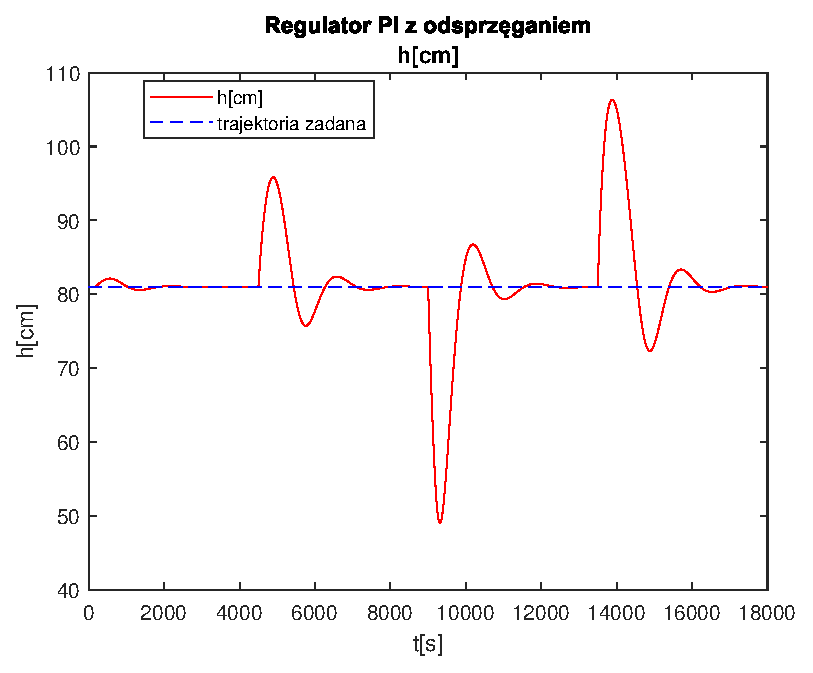
\includegraphics[width=1\linewidth]{img/PI/decoupler/disturbance/PIDecouplerH2DisttrueLinfalse.eps}
      \caption{}
      \label{fig:fig:PIDecoupler2DisttrueLinfalse1}
   \end{subfigure}
       
   \begin{subfigure}[b]{0.4\textwidth}
      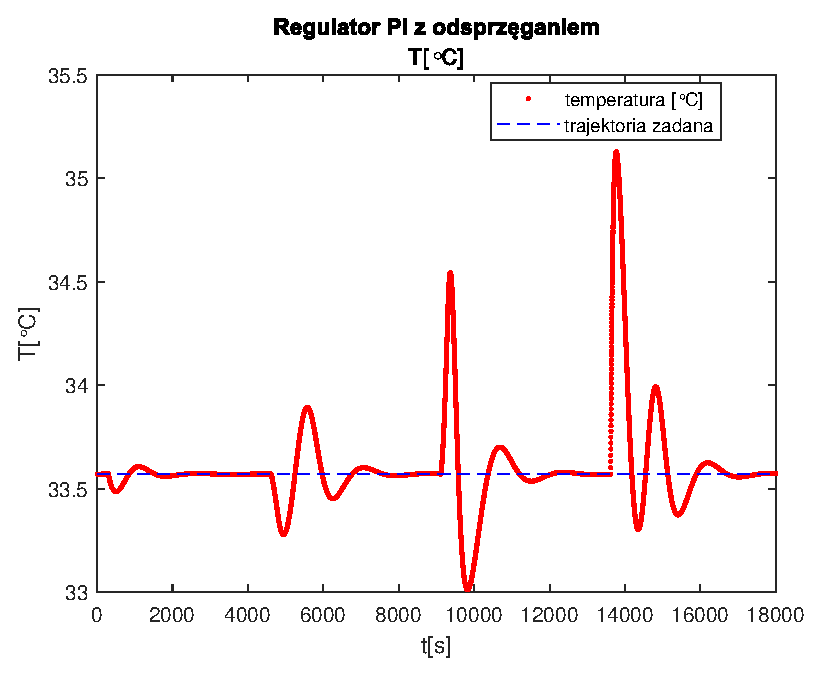
\includegraphics[width=1\linewidth]{img/PI/decoupler/disturbance/PIDecouplerT2DisttrueLinfalse.eps}
      \caption{}
      \label{fig:fig:PIDecoupler2DisttrueLinfalse2}
   \end{subfigure}
       
   \begin{subfigure}[b]{0.4\textwidth}
      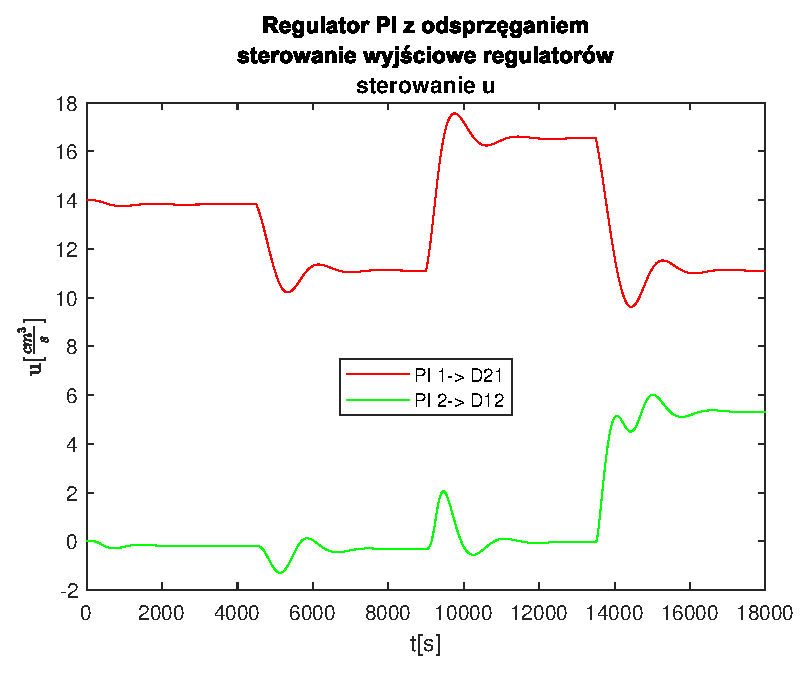
\includegraphics[width=1\linewidth]{img/PI/decoupler/disturbance/PIDecouplerControlD2DisttrueLinfalse.eps}
      \caption{}
      \label{fig:fig:PIDecoupler2DisttrueLinfalse3}
   \end{subfigure}
       
   \begin{subfigure}[b]{0.4\textwidth}
      \includegraphics[width=1\linewidth]{img/PI/decoupler/disturbance/PIDecouplerDisturbance2DisttrueLinfalse.eps}
      \caption{}
      \label{fig:fig:PIDecoupler2DisttrueLinfalse4}
   \end{subfigure}
       
   \caption{Wykresy dla regulatora PI z odsprzeganiem dla różnych wartości zakłóceń}
   \label{fig:PIDecoupler2DisttrueLinfalse}
\end{figure}
           
\begin{figure}[h!]
   \centering
   \begin{subfigure}[b]{0.4\textwidth}
      \includegraphics[width=1\linewidth]{img/PI/decoupler/disturbance/PIDecouplerH3DisttrueLinfalse.eps}
      \caption{}
      \label{fig:fig:PIDecoupler3DisttrueLinfalse1}
   \end{subfigure}
       
   \begin{subfigure}[b]{0.4\textwidth}
      \includegraphics[width=1\linewidth]{img/PI/decoupler/disturbance/PIDecouplerT3DisttrueLinfalse.eps}
      \caption{}
      \label{fig:fig:PIDecoupler3DisttrueLinfalse2}
   \end{subfigure}
       
   \begin{subfigure}[b]{0.4\textwidth}
      \includegraphics[width=1\linewidth]{img/PI/decoupler/disturbance/PIDecouplerControlD3DisttrueLinfalse.eps}
      \caption{}
      \label{fig:fig:PIDecoupler3DisttrueLinfalse3}
   \end{subfigure}
       
   \begin{subfigure}[b]{0.4\textwidth}
      \includegraphics[width=1\linewidth]{img/PI/decoupler/disturbance/PIDecouplerDisturbance3DisttrueLinfalse.eps}
      \caption{}
      \label{fig:fig:PIDecoupler3DisttrueLinfalse4}
   \end{subfigure}
       
   \caption{Wykresy dla regulatora PI z odsprzeganiem dla różnych wartości zakłóceń}
   \label{fig:PIDecoupler3DisttrueLinfalse}
\end{figure}
           

\FloatBarrier

\subsection{Napełniania zbiornika do punktu pracy PI z modelem nieliniowym}
\indent Sprawdzając jak zachowa się układ dla napełniania zbiornika przy użyciu odprzęgania można zauważyć, że układ regulacji radzi sobie zdecydowanie lepiej niż w przypadku bez odprzęgania. Występujące prze regulowania są znikome i szybko zostają stłumione. Z charakterystyk sterowania widać, że regulator odpowiadający za dopływ zimnej wody daje na wyjściu daje wartości ujemne. Jednak człon odprzęgający koryguje tą zależność na podstawie wyliczonego dopływu ciepłej wody. Zatem charakterystyka sygnału sterującego w stanie ustalonym daję dość szybko sygnały sterujące w punkcie pracy.
\FloatBarrier
    \begin{figure}[h!]
   \centering
   \begin{subfigure}[b]{0.4\textwidth}
      \includegraphics[width=1\linewidth]{img/PI/decoupler/noDisturbance/PIDecouplerH0.eps}
      \caption{}
      \label{fig:fig:PIDecoupler01}
   \end{subfigure}
       
   \begin{subfigure}[b]{0.4\textwidth}
      \includegraphics[width=1\linewidth]{img/PI/decoupler/noDisturbance/PIDecouplerT0.eps}
      \caption{}
      \label{fig:fig:PIDecoupler02}
   \end{subfigure}
       
   \begin{subfigure}[b]{0.4\textwidth}
      \includegraphics[width=1\linewidth]{img/PI/decoupler/noDisturbance/PIDecouplerControl0.eps}
      \caption{}
      \label{fig:fig:PIDecoupler03}
   \end{subfigure}
       
   \begin{subfigure}[b]{0.4\textwidth}
      \includegraphics[width=1\linewidth]{img/PI/decoupler/noDisturbance/PIDecouplerControlD0.eps}
      \caption{}
      \label{fig:fig:PIDecoupler04}
   \end{subfigure}
       
   \caption{Wykresy dla regulatora PI z odsprzeganiem.}
   \label{fig:PIDecoupler0}
\end{figure}
           

\FloatBarrier
\newpage
\section{Analityczny regulator predykcyjny MPCS}
Do obliczeń regulatora predykcyjnego MPCS wykorzystano model liniowy obiektu w oparciu o równania stanu postaci zgodnej z równaniem \ref{equation:defaultdss}. Wektor stanu $x$ i wejścia $u$ odpowiadał zmiennym zgodnie z równaniem \ref{equation:defineddss}. Po wykonaniu obliczeń, współczynniki macierzy $A$, $B$, $C$, oraz $D$ wynosiły tyle ile na równaniu \ref{equation:matricesdvals}. Zmienna $k_{const_0}$ odpowiada dodatkowej stałej dodawanej do obliczeń objętości, jest ona nieistotna dla pracy regulatora. Należy zauważyć, że zmienną wyjściową modelu jest zmienna $V$. Ponieważ znana jest zależność między $V$ a $H$, zamiana z jednej zmiennej na drugą jest prosta. Pojawia się za to problem uwarunkowania macierzy $B$. Wartości objętości są o około 2 rzędy większe niż wartości temperatury. Dlatego regulator wykonuje obliczenia na modelu o $100$ krotnie zmniejszonej objętości, a więc także o $100$ krotnie zmniejszonym pierwszym wersie macierzy $B$, regulator nie bierze również pod uwagę wejść niesterowalnych, macierz $B$ wykorzystywana przez regulator ma więc postać $B_{reg}$, zgodnie ze wzorem \ref{equation:bregval}. Ogólna struktura regulacji przedstawiona jest na Rys. \ref{fig:mpcs}. Na wykresach pokazane jest działanie regulatora dla przykładowego przebiegu wartości zadanych, różnych wartości horyzontów $N$ i $N_u$, oraz parametru $\lambda$, dla obiektu określonego liniowymi równaniami stanu oraz dla obiektu nieliniowego zdyskretyzowanego metodą rk4. Przyjęto wartości sterowania w zakresie $\langle 0 : 100 \rangle$, oraz maksymalną zmianę sterowania w jednej chwili $k$ za $\pm0.2$. Należy zauważyć, że zmienna $T$ obarczona jest znacznym błędem linearyzacji. Jak można zauważyć na podstawie wykresów, regulator MPCS charakteryzuje się niewielkim uchybem ustalonym dla zmiennej $T$, może on wynikać z błędu linearyzacji. Poza tym problemem, regulator działa bardzo dobrze nawet z ograniczeniami, dla horyzontów o wartościach na poziomie kilkuset próbek. Wartości zmiennych sterowanych szybko zbiegają do wartości zadanych, a przeregulowania są względnie niewielkie. Dla dużych zmian wartości zadanych jednak regulator ten nie może być dobrze zastosowany, ze względu na błędy wynikające z linearyzacji obiektu. Oczywiście obiekt oparty o równania przestrzeni stanu nie jest obarczony tymi problemami i regulacja w jego przypadku jest niemal idealna. Na ostatnim wykresie przedstawiono również działanie regulatora dla zmiennego zakłócenia $F_d$. Jak widać, nie radzi on sobie zbyt dobrze ze zmiennym zakłóceniem.


\begin{equation}
\label{equation:defaultdss}
\begin{aligned}
    x(k+1) = & Ax(k) + Bu(k) \\
    y(k) = & Cx(k) + Du(k)
\end{aligned}
\end{equation}

\begin{equation}
\label{equation:defineddss}
    \begin{aligned}
        x = &
        \begin{bmatrix}
            V \\
            T 
        \end{bmatrix}\\
        u = &
        \begin{bmatrix}
            F_H \\
            F_C \\
            F_D \\
            T_H \\
            T_C \\
            T_D
        \end{bmatrix}
    \end{aligned}
\end{equation}

\begin{equation}
\label{equation:matricesdvals}
    \begin{aligned}
        k_{const_0} &= -47.25\\
        A = &
        \begin{bmatrix}
            0.9966 & 0\\
            -4.23e-09 & 0.9864\\
        \end{bmatrix} \\
        B = &
        \begin{bmatrix}
            0.9983 & 0.9983 & 0.9983 & 0 & 0 & 0\\
            0.006148 & -0.002286 & -0.0001233 & 0.003028 & 0.008001 & 0.002595\\
        \end{bmatrix}\\
        C = &
        \begin{bmatrix}
            1 & 0\\
            0 & 1
        \end{bmatrix}\\
        D = & 
        \begin{bmatrix}
            0 & 0 & 0 & 0 & 0 & 0 \\
            0 & 0 & 0 & 0 & 0 & 0 
        \end{bmatrix}
    \end{aligned}
\end{equation}

\begin{equation}
\label{equation:bregval}
    \begin{aligned}
        B_{reg} = &
        \begin{bmatrix}
            0.009983 & 0.009983\\
            0.006148 & -0.002286\\
        \end{bmatrix}\\
    \end{aligned}
\end{equation}

\begin{figure}[h!]
   \centering
   \includegraphics[scale=0.7]{img/MPCSanaRK/MPCSDiag.pdf}
   \caption{Ogólny schemat regulacji z wykorzystaniem algorytmu MPCS}
   \label{fig:mpcs}
\end{figure}


\FloatBarrier
    \begin{figure}[h!]
   \centering
   \begin{subfigure}[b]{0.4\textwidth}
      \includegraphics[width=1\linewidth]{img/MPCSanaRK/MPCSRKHN50Nu10l100.eps}
      \caption{}
      \label{fig:fig:MPCSRKN50Nu10l1001}
   \end{subfigure}
       
   \begin{subfigure}[b]{0.4\textwidth}
      \includegraphics[width=1\linewidth]{img/MPCSanaRK/MPCSRKTN50Nu10l100.eps}
      \caption{}
      \label{fig:fig:MPCSRKN50Nu10l1002}
   \end{subfigure}
       
   \begin{subfigure}[b]{0.4\textwidth}
      \includegraphics[width=1\linewidth]{img/MPCSanaRK/MPCSRKControlN50Nu10l100.eps}
      \caption{}
      \label{fig:fig:MPCSRKN50Nu10l1003}
   \end{subfigure}
       
   \caption{Wykresy dla regulatora MPCS, obiekt nieliniowy, $N = 50$, $N_u = 10$, $\lambda = 1$ .}
   \label{fig:MPCSRKN50Nu10l100}
\end{figure}
           

\FloatBarrier

\FloatBarrier
    \begin{figure}[h!]
   \centering
   \begin{subfigure}[b]{0.4\textwidth}
      \includegraphics[width=1\linewidth]{img/MPCSanaLin/MPCSLinHN300Nu100l10.eps}
      \caption{}
      \label{fig:fig:MPCSLinN300Nu100l101}
   \end{subfigure}
       
   \begin{subfigure}[b]{0.4\textwidth}
      \includegraphics[width=1\linewidth]{img/MPCSanaLin/MPCSLinTN300Nu100l10.eps}
      \caption{}
      \label{fig:fig:MPCSLinN300Nu100l102}
   \end{subfigure}
       
   \begin{subfigure}[b]{0.4\textwidth}
      \includegraphics[width=1\linewidth]{img/MPCSanaLin/MPCSLinControlN300Nu100l10.eps}
      \caption{}
      \label{fig:fig:MPCSLinN300Nu100l103}
   \end{subfigure}
       
   \caption{Wykresy dla regulatora MPCS, obiekt liniowy, $N = 300$, $N_u = 100$, $\lambda = 0.1$.}
   \label{fig:MPCSLinN300Nu100l10}
\end{figure}
           

\FloatBarrier

\FloatBarrier
    \begin{figure}[h!]
   \centering
   \begin{subfigure}[b]{0.4\textwidth}
      \includegraphics[width=1\linewidth]{img
\FloatBarrier

\FloatBarrier
    \begin{figure}[h!]
   \centering
   \begin{subfigure}[b]{0.4\textwidth}
      \includegraphics[width=1\linewidth]{img/MPCSanaLin/MPCSLinHN300Nu100l10.eps}
      \caption{}
      \label{fig:fig:MPCSLinN300Nu100l101}
   \end{subfigure}
       
   \begin{subfigure}[b]{0.4\textwidth}
      \includegraphics[width=1\linewidth]{img/MPCSanaLin/MPCSLinTN300Nu100l10.eps}
      \caption{}
      \label{fig:fig:MPCSLinN300Nu100l102}
   \end{subfigure}
       
   \begin{subfigure}[b]{0.4\textwidth}
      \includegraphics[width=1\linewidth]{img/MPCSanaLin/MPCSLinControlN300Nu100l10.eps}
      \caption{}
      \label{fig:fig:MPCSLinN300Nu100l103}
   \end{subfigure}
       
   \caption{Wykresy dla regulatora MPCS, obiekt liniowy, $N = 300$, $N_u = 100$, $\lambda = 0.1$.}
   \label{fig:MPCSLinN300Nu100l10}
\end{figure}
           

\FloatBarrier

\FloatBarrier
    \begin{figure}[h!]
   \centering
   \begin{subfigure}[b]{0.4\textwidth}
      \includegraphics[width=1\linewidth]{img/MPCSanaRK/MPCSRKHN500Nu60l40.eps}
      \caption{}
      \label{fig:fig:MPCSRKN500Nu60l401}
   \end{subfigure}
       
   \begin{subfigure}[b]{0.4\textwidth}
      \includegraphics[width=1\linewidth]{img/MPCSanaRK/MPCSRKTN500Nu60l40.eps}
      \caption{}
      \label{fig:fig:MPCSRKN500Nu60l402}
   \end{subfigure}
       
   \begin{subfigure}[b]{0.4\textwidth}
      \includegraphics[width=1\linewidth]{img/MPCSanaRK/MPCSRKControlN500Nu60l40.eps}
      \caption{}
      \label{fig:fig:MPCSRKN500Nu60l403}
   \end{subfigure}
       
   \caption{Wykresy dla regulatora MPCS, obiekt nieliniowy.}
   \label{fig:MPCSRKN500Nu60l40}
\end{figure}
           

\FloatBarrier

\FloatBarrier
    \begin{figure}[h!]
   \centering
   \begin{subfigure}[b]{0.4\textwidth}
      \includegraphics[width=1\linewidth]{img/MPCSanaLin/MPCSLinHN500Nu60l40.eps}
      \caption{}
      \label{fig:fig:MPCSLinN500Nu60l401}
   \end{subfigure}
       
   \begin{subfigure}[b]{0.4\textwidth}
      \includegraphics[width=1\linewidth]{img/MPCSanaLin/MPCSLinTN500Nu60l40.eps}
      \caption{}
      \label{fig:fig:MPCSLinN500Nu60l402}
   \end{subfigure}
       
   \begin{subfigure}[b]{0.4\textwidth}
      \includegraphics[width=1\linewidth]{img/MPCSanaLin/MPCSLinControlN500Nu60l40.eps}
      \caption{}
      \label{fig:fig:MPCSLinN500Nu60l403}
   \end{subfigure}
       
   \caption{Wykresy dla regulatora MPCS, obiekt liniowy, $N = 500$, $N_u = 60$, $\lambda = 0.4$.}
   \label{fig:MPCSLinN500Nu60l40}
\end{figure}
           

\FloatBarrier
\newpage
\section{Porównanie dwupętlowego regulatora PI z analitycznym regulatorem MPCS}
\indent W poniższych podrozdziałach zostaną zaprezentowane podobieństwa i różnice pomiędzy analitycznym regulatorem MPCS i dwupętlowym PI. Wynika z nich, że jeśli dysponuje się małą mocą obliczeniową lepszy rozwiązaniem będzie prosty PI. Jeśli ma się do dyspozycji bardziej wydajny sprzęt i jest taka potrzeba podczas produkcji wskazane jest użycie regulatora predykcyjnego.
\subsection{Podobieństwa}
\indent Dla obu zmiana zadanej wartości wyjścia sprawia, że na drugim wyjściu pojawia się uchyb.
\indent Oba regulatory są w stanie odpowiednio ustawić sterowania, by osiągnąć wartości zadane.
\indent Oba są podatne na błędy linearyzacji.
\subsection{Różnice}
\begin{itemize}
    \item Regulator PI działa zdecydowanie szybciej i wymaga mniejszej mocy obliczeniowej
    \item Regulator PI ma generalnie większe wartości uchybów na wyjściu drugim wyjściu po zmianie wartości zadanej na pierwszym wyjściu.
    \item Sygnały sterujące dla regulatora predykcyjnego są mniej rozmyte, tzn regulator szybciej dobiera odpowiednią wartość sterowania dla wartości zadanej.
\end{itemize}
\newpage
\section{Numeryczny regulator predykcyjny MPCS}
\indent W numerycznym regulatorze w każdej chwili $k$ rozwiązywane jest zadanie programowania kwadratowego, które uwzględnia ograniczenia sterowania. Znacznie zwiększa to już i tak dosyć długi czas obliczeń, dlatego przedstawione zostały jedynie przypadki tych regulatorów dla niewielkich wartości horyzontów, przez co jakość regulacji jest względnie niska. Musi również istnieć rozwiązanie quadprog dla danych trajektorii wartości zadanych, zostały więc one zmienione, żeby sterowanie było nieco prostsze. \\ \indent Wykresy przedstawiają działanie regulatora analitycznego oraz numerycznego dla takich samych parametrów regulatora. Regulator numeryczny działał zauważalnie lepiej dla wyjścia $V$, ale radził sobie nieco gorzej z opóźnieniami na wyjściu $T$, należy również zauważyć, że ze względu na krótszy czas obliczeń, regulator analityczny może brać pod uwagę większą ilość elementów odpowiedzi skokowej, podczas gdy regulator numeryczny działa z akceptowalną częstotliwością próbkowania jedynie dla względnie niskich horyzontów predykcji, przez co w rzeczywistości regulator analityczny może się sprawdzać lepiej. Regulatory działały z obiektem nieliniowym.



\FloatBarrier
    \begin{figure}[h!]
   \centering
   \begin{subfigure}[b]{0.4\textwidth}
      \includegraphics[width=1\linewidth]{img/MPCSnumRK/MPCSRKHN100Nu50l50.eps}
      \caption{}
      \label{fig:fig:MPCSRKN100Nu50l501}
   \end{subfigure}
       
   \begin{subfigure}[b]{0.4\textwidth}
      \includegraphics[width=1\linewidth]{img/MPCSnumRK/MPCSRKTN100Nu50l50.eps}
      \caption{}
      \label{fig:fig:MPCSRKN100Nu50l502}
   \end{subfigure}
       
   \begin{subfigure}[b]{0.4\textwidth}
      \includegraphics[width=1\linewidth]{img/MPCSnumRK/MPCSRKControlN100Nu50l50.eps}
      \caption{}
      \label{fig:fig:MPCSRKN100Nu50l503}
   \end{subfigure}
       
   \caption{Wykresy dla regulatora MPCS, obiekt nieliniowy, $N = 100$, $N_u = 50$.}
   \label{fig:MPCSRKN100Nu50l50}
\end{figure}
           

\FloatBarrier

\FloatBarrier
    \begin{figure}[h!]
   \centering
   \begin{subfigure}[b]{0.4\textwidth}
      \includegraphics[width=1\linewidth]{img/MPCSnumRK/MPCSRKHN50Nu10l20.eps}
      \caption{}
      \label{fig:fig:MPCSRKN50Nu10l201}
   \end{subfigure}
       
   \begin{subfigure}[b]{0.4\textwidth}
      \includegraphics[width=1\linewidth]{img/MPCSnumRK/MPCSRKTN50Nu10l20.eps}
      \caption{}
      \label{fig:fig:MPCSRKN50Nu10l202}
   \end{subfigure}
       
   \begin{subfigure}[b]{0.4\textwidth}
      \includegraphics[width=1\linewidth]{img/MPCSnumRK/MPCSRKControlN50Nu10l20.eps}
      \caption{}
      \label{fig:fig:MPCSRKN50Nu10l203}
   \end{subfigure}
       
   \caption{Wykresy dla regulatora MPCS, obiekt nieliniowy, $N = 50$, $N_u = 10$, $\lambda = 0.2$.}
   \label{fig:MPCSRKN50Nu10l20}
\end{figure}
           

\FloatBarrier

\FloatBarrier
    \begin{figure}[h!]
   \centering
   \begin{subfigure}[b]{0.4\textwidth}
      \includegraphics[width=1\linewidth]{img/MPCSnumRK/MPCSRKHN80Nu30l30.eps}
      \caption{}
      \label{fig:fig:MPCSRKN80Nu30l301}
   \end{subfigure}
       
   \begin{subfigure}[b]{0.4\textwidth}
      \includegraphics[width=1\linewidth]{img/MPCSnumRK/MPCSRKTN80Nu30l30.eps}
      \caption{}
      \label{fig:fig:MPCSRKN80Nu30l302}
   \end{subfigure}
       
   \begin{subfigure}[b]{0.4\textwidth}
      \includegraphics[width=1\linewidth]{img/MPCSnumRK/MPCSRKControlN80Nu30l30.eps}
      \caption{}
      \label{fig:fig:MPCSRKN80Nu30l303}
   \end{subfigure}
       
   \caption{Wykresy dla regulatora MPCS, obiekt nieliniowy, $N = 80$, $N_u = 30$, $\lambda = 0.3$.}
   \label{fig:MPCSRKN80Nu30l30}
\end{figure}
           

\FloatBarrier
\newpage
\section{Porównanie numerycznej i analitycznej wersji MPCS}
\subsection{Podobieństwa}
\begin{itemize}
    \item Dla niskich wartości horyzontów predykcji zbiegają dosyć wolno do wartości zadanej
    \item Wysoka złożoność obliczeniowa
    \item Dobre działanie dla odpowiednio dobranych parametrów
    \item Brak sprzężenia zwrotnego, podatność na błędy linearyzacji
    \item W ogólności powinny działać lepiej niż PI
\end{itemize}
\subsection{Różnice}
\begin{itemize}
    \item Wersja numeryczna ma niewielkie przeregulowania i niewielkie oscylacje dla niskich wartości horyzontów, analityczna mocno dla nich oscyluje
    \item Wersja analityczna działa nieco lepiej dla niskich opóźnień, a wersja numeryczna nieco lepiej dla wysokich opóźnień
    \item Pomimo iż oba są wymagające obliczeniowo, wersja numeryczna wymaga znacznie większej ilości obliczeń niż wersja analityczna
\end{itemize}

\end{document}
